\documentclass[10pt,winfonts,fancyhdr,hyperref,UTF8]{ctexrep}
\usepackage{indentfirst} 
\usepackage{fontspec}
\usepackage{titlesec}
\usepackage{xeCJK}
\usepackage{graphicx}
\usepackage{ifthen}
\usepackage{color,fancyvrb}
\usepackage{listings}
\usepackage{syntonly}
\usepackage{makeidx}
\usepackage[hidelinks, colorlinks=true]{hyperref}
\usepackage{algorithm}
\usepackage{algpseudocode}
\usepackage{amssymb}
\usepackage{multirow}
\usepackage{ulem}
\usepackage{diagbox}
\makeatletter
%LeetCode Setting
\usepackage[centering,paperwidth=180mm,paperheight=230mm,%
body={390pt,530pt},marginparsep=10pt,marginpar=50pt]{geometry}
\usepackage{color}
\usepackage{enumitem}
\usepackage{fancyvrb}
\usepackage[bottom,perpage,symbol*]{footmisc}
\usepackage{graphicx}
\usepackage[hidelinks]{hyperref}
\usepackage{makeidx}
\usepackage[toc]{multitoc}
\usepackage{pifont}
\usepackage{underscore}
\usepackage{amsmath}

\DefineFNsymbols*{chinese}{{\ding{172}}{\ding{173}}{\ding{174}}{\ding{175}}%
{\ding{176}}{\ding{177}}{\ding{178}}{\ding{179}}{\ding{180}}{\ding{181}}}
\setfnsymbol{chinese}

\hypersetup{bookmarksnumbered=true,bookmarksdepth=2}

\CTEXsetup[number={\thechapter}]{chapter}
\CTEXsetup[format+={\raggedleft}]{chapter}
\CTEXsetup[beforeskip={10pt}]{chapter}
\CTEXsetup[afterskip={30pt}]{chapter}
\def\CTEX@chapter@aftername{\par} % \CTEXsetup[aftername={\par}]{chapter}
\CTEXsetup[format+={\raggedright}]{section}
\CTEXsetup[beforeskip={-3.0ex plus -1ex minus -.2ex}]{section}
\CTEXsetup[afterskip={2.3ex plus .2ex minus 0.2ex}]{section}

\renewcommand \thefigure{\thechapter-\arabic{figure}}
\renewcommand \thetable{\thechapter-\arabic{table}}

\newcommand\figcaption[1]{\def\@captype{figure}\caption{#1}}
\newcommand\tabcaption[1]{\def\@captype{table}\caption{#1}}

\long\def\@caption#1[#2]#3{%
  \addcontentsline{\csname ext@#1\endcsname}{#1}%
    {\protect\numberline{\csname fnum@#1\endcsname}{ \ignorespaces #2}}% change "the" to "fnum@"
    \normalsize
    \@makecaption{\csname fnum@#1\endcsname}{\ignorespaces #3}}

\long\def\@makecaption#1#2{%
  \vskip\abovecaptionskip
  \sbox\@tempboxa{#1\quad#2}%
  \ifdim \wd\@tempboxa >\hsize
    #1\quad#2\par
  \else
    \global \@minipagefalse
    \hb@xt@\hsize{\hfil\box\@tempboxa\hfil}%
  \fi
  \vskip\belowcaptionskip}

\setlength\abovecaptionskip{0pt}
  
\setmainfont{Times New Roman}
%\setmainfont{Linux Libertine}
%\setmainfont{TeX Gyre Pagella}
\newfontfamily\urlfont{Times New Roman}
%\setmonofont[AutoFakeBold=1.6,AutoFakeSlant=0.17,Mapping=tex-text-tt]{Inconsolata}
\setCJKfamilyfont{zhyou}{YouYuan}

\newcommand{\fn}[1]{\texttt{#1}}
\newcommand{\sfn}[1]{\texttt{\small #1}}
\newcommand{\kw}[1]{\textsf{#1}}
\newcommand{\myurl}[1]{{\urlfont #1}}
\newcommand{\mpar}[1]{\marginpar[\hfill\kaishu #1]{\kaishu #1}}
\newcommand{\mn}[1]{\texttt{\bs #1}}
\renewcommand{\today}{\the\year-\the\month-\the\day}
\newcommand\bs{\textbackslash}
\newcommand{\code}[1]{\small{\fontspec{Latin Modern Mono} #1}}

\newcommand\begindot{\begin{itemize}
[itemsep=2pt plus 2pt minus 2pt,%
topsep=3pt plus 2pt minus 2pt,%
parsep=0pt plus 2pt minus 2pt]}
\newcommand\myenddot{\end{itemize}}

\newcommand\beginnum{\begin{enumerate}
[itemsep=2pt plus 2pt minus 2pt,%
topsep=3pt plus 2pt minus 2pt,%
parsep=0pt plus 2pt minus 2pt]}
\newcommand\myendnum{\end{enumerate}}

\DefineVerbatimEnvironment%
  {Code}{Verbatim}
  {fontsize=\small,baselinestretch=0.9,xleftmargin=3mm}

\raggedbottom
%\setlength{\parskip}{1ex plus .5ex minus .5ex}

\def\FV@SetLineWidth{%
  \if@FV@ResetMargins\else
    \advance\leftmargin\@totalleftmargin
  \fi
  \advance\leftmargin\FV@XLeftMargin\relax
  \advance\rightmargin\FV@XRightMargin\relax
  \linewidth\hsize
  %\advance\linewidth-\leftmargin
  %\advance\linewidth-\rightmargin
  \hfuzz\FancyVerbHFuzz\relax}


\def\FV@SingleFrameLine#1{%
%% DG/SR modification end
  \hbox to\z@{%
    %\kern\leftmargin
%% DG/SR modification begin - Jun. 22, 1998
    \ifnum#1=\z@
      \let\FV@Label\FV@LabelBegin
    \else
      \let\FV@Label\FV@LabelEnd
    \fi
    \ifx\FV@Label\relax
%% DG/SR modification end
      \FancyVerbRuleColor{\vrule \@width\linewidth \@height\FV@FrameRule}%
%% DG/SR modification begin - Jun. 22, 1998
    \else
      \ifnum#1=\z@
        \setbox\z@\hbox{\strut\enspace\urlfont\FV@LabelBegin\strut}%
      \else
        \setbox\z@\hbox{\strut\enspace\urlfont\FV@LabelEnd\strut}%
      \fi
      \@tempdimb=\dp\z@
      \advance\@tempdimb -.5\ht\z@
      \@tempdimc=\linewidth
      \advance\@tempdimc -\wd\z@
      %\divide\@tempdimc\tw@
      \ifnum#1=\z@              % Top line
        \ifx\FV@LabelPositionTopLine\relax
          \FancyVerbRuleColor{\vrule \@width\linewidth \@height\FV@FrameRule}%
        \else
          \FV@FrameLineWithLabel
        \fi
      \else                     % Bottom line
        \ifx\FV@LabelPositionBottomLine\relax
          \FancyVerbRuleColor{\vrule \@width\linewidth \@height\FV@FrameRule}%
        \else
          \FV@FrameLineWithLabel
        \fi
      \fi
    \fi
%% DG/SR modification end
    \hss}}


%% DG/SR modification begin - May. 19, 1998
\def\FV@FrameLineWithLabel{%
  \ht\z@\@tempdimb\dp\z@\@tempdimb%
  \FancyVerbRuleColor{%
    \raise 0.5ex\hbox{\vrule \@width\@tempdimc \@height\FV@FrameRule}%
    \raise\@tempdimb\box\z@}}
%% DG/SR modification end


\def\FV@EndListFrame@Lines{%
  \begingroup
    %\vskip 0.5ex
    \baselineskip\z@skip
    \kern\FV@FrameSep\relax
%% DG/SR modification begin - May. 19, 1998
%%    \FV@SingleFrameLine
    \FV@SingleFrameLine{\@ne}%
%% DG/SR modification end
  \endgroup}

\newskip\mytopsep
\setlength{\mytopsep}{4pt plus 2pt minus 3pt}

\def\FV@ListVSpace{%
  \@topsepadd\mytopsep
  \if@noparlist\advance\@topsepadd\partopsep\fi
  \if@inlabel
    \vskip\parskip
  \else
    \if@nobreak
      \vskip\parskip
      \clubpenalty\@M
    \else
      \addpenalty\@beginparpenalty
      \@topsep\@topsepadd
      \advance\@topsep\parskip
      \addvspace\@topsep
    \fi
  \fi
  %\showthe \@topsepadd
  %\showthe \topsep
  %\showthe \partopsep
  %\showthe \parskip
  \global\@nobreakfalse
  \global\@inlabelfalse
  \global\@minipagefalse
  \global\@newlistfalse}

\def\FV@EndList{%
  \FV@ListProcessLastLine
  \FV@EndListFrame
  %\showthe \@topsepadd
  \@endparenv
  \endgroup
  \@endpetrue}

\def\theFancyVerbLine{\sffamily\scriptsize\arabic{FancyVerbLine}}

\DefineVerbatimEnvironment%
  {Codex}{Verbatim}
  {fontsize=\small,baselinestretch=0.9,xleftmargin=3mm,%
  frame=lines,labelposition=all,framesep=5pt}

\DefineVerbatimEnvironment%
  {Code}{Verbatim}
  {fontsize=\small,baselinestretch=0.9,xleftmargin=3mm}

\makeindex

%Other settings:
\lstset{%  
  alsolanguage=Java,  
  language={C++},
  tabsize=4, %  
  frame=shadowbox, %把代码用带有阴影的框圈起来  
  commentstyle=\color{red!50!green!50!blue!50},%浅灰色的注释  
  rulesepcolor=\color{red!20!green!20!blue!20},%代码块边框为淡青色  
  keywordstyle=\color{blue!90}\bfseries, %代码关键字的颜色为蓝色,粗体  
  showstringspaces=false,%不显示代码字符串中间的空格标记  
  stringstyle=\ttfamily, % 代码字符串的特殊格式  
  keepspaces=true, %  
  breakindent=22pt, %  
  numbers=left,%左侧显示行号 往左靠,还可以为right,或none,即不加行号  
  stepnumber=1,%若设置为2,则显示行号为1,3,5,即stepnumber为公差,默认stepnumber=1  
  %numberstyle=\tiny, %行号字体用小号  
  numberstyle={\color[RGB]{0,192,192}\tiny} ,%设置行号的大小,大小有tiny,scriptsize,footnotesize,small,normalsize,large等  
  numbersep=8pt,  %设置行号与代码的距离,默认是5pt  
  basicstyle=\footnotesize, % 这句设置代码的大小  
  showspaces=false, %  
  flexiblecolumns=true, %  
  breaklines=true, %对过长的代码自动换行  
  breakautoindent=true,%  
  breakindent=4em, %  
  aboveskip=1em, %代码块边框  
  tabsize=2,  
  showstringspaces=false, %不显示字符串中的空格  
  backgroundcolor=\color[RGB]{245,245,244},   %代码背景色  
}















\makeatother
%\graphicspath{{images/}}

\usepackage{tikz}
\usetikzlibrary{calc}
\usetikzlibrary{fit}
\usetikzlibrary{positioning}
\usepgflibrary{plotmarks}

\usetikzlibrary{shapes.geometric}

\CustomVerbatimEnvironment{shellcmd}{Verbatim}
{frame=single,rulecolor=\color{blue},framerule=3pt,framesep=1pc,fillcolor=\color{yellow}}

\newcommand{\bookname}{TechNotes}
\renewcommand{\contentsname}{OS} 

\title{\sffamily OS}
\date{\today}
\setcounter{tocdepth}{1}
\setcounter{chapter}{12}

\begin{document}

%\maketitle
\tableofcontents


%TOADD
%!Mode:: "TeX:UTF-8"
 \chapter{操作系统}

%!Mode:: "TeX:UTF-8"

\section{进程}

\subsection{进程与线程}
进程的四大特征:\textbf{动态性,并发性,独立性,异步性}。

进程与程序的关系:一个进程可以依次执行多个程序,多个进程可共同执行一个程序。

进程与线程的区别:
从内核的观点看,进程的目的就是担当分配系统资源(CPU时间、内存等)的基本单位。线程是进程的一个执行流,是CPU调度和分派的基本单位,它是比进程更小的能独立运行的基本单位。

进程是独立的,这表现在内存空间、上下文环境上;线程运行在进程空间内。一般来讲(不使用特殊技术),进程无法突破进程边界存取其他进程的存储空间;
而线程由于处于进程空间内,所有同一进程的线程共享同一内存空间。

线程是属于进程的,当进程退出时该进程所产生的线程都会被强制退出并清除。线程所占用的资源要少于进程所占用的资源。进程和线程都可以有优先级。

\textbf{多进程和多线程各有什么优缺点}?
进程优点:编程、调试简单,可靠性较高,适合多机、多核系统。\\
线程优点:创建、销毁、切换速度快,内存、资源占用小,数据共享简单,只适合多核系统。

\subsection{进程内存布局}
图\ref{fig:processmemlayout}为典型的内存布局(选择《APUE》)。
\begin{figure}[ht]
	\begin{center}
		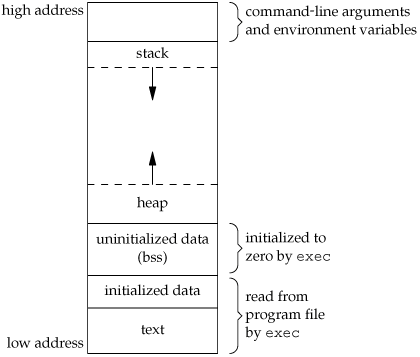
\includegraphics[keepaspectratio,width=0.5\paperwidth]{Pictures/Kernel/programMemLayout.png}
	\caption{进程的典型内存布局示例}
	\label{fig:processmemlayout}
	\end{center}
\end{figure}

《CSAPP》给出的内存布局如图\ref{fig:processmemlayout-csapp}所示。
\begin{figure}[ht]
	\begin{center}
		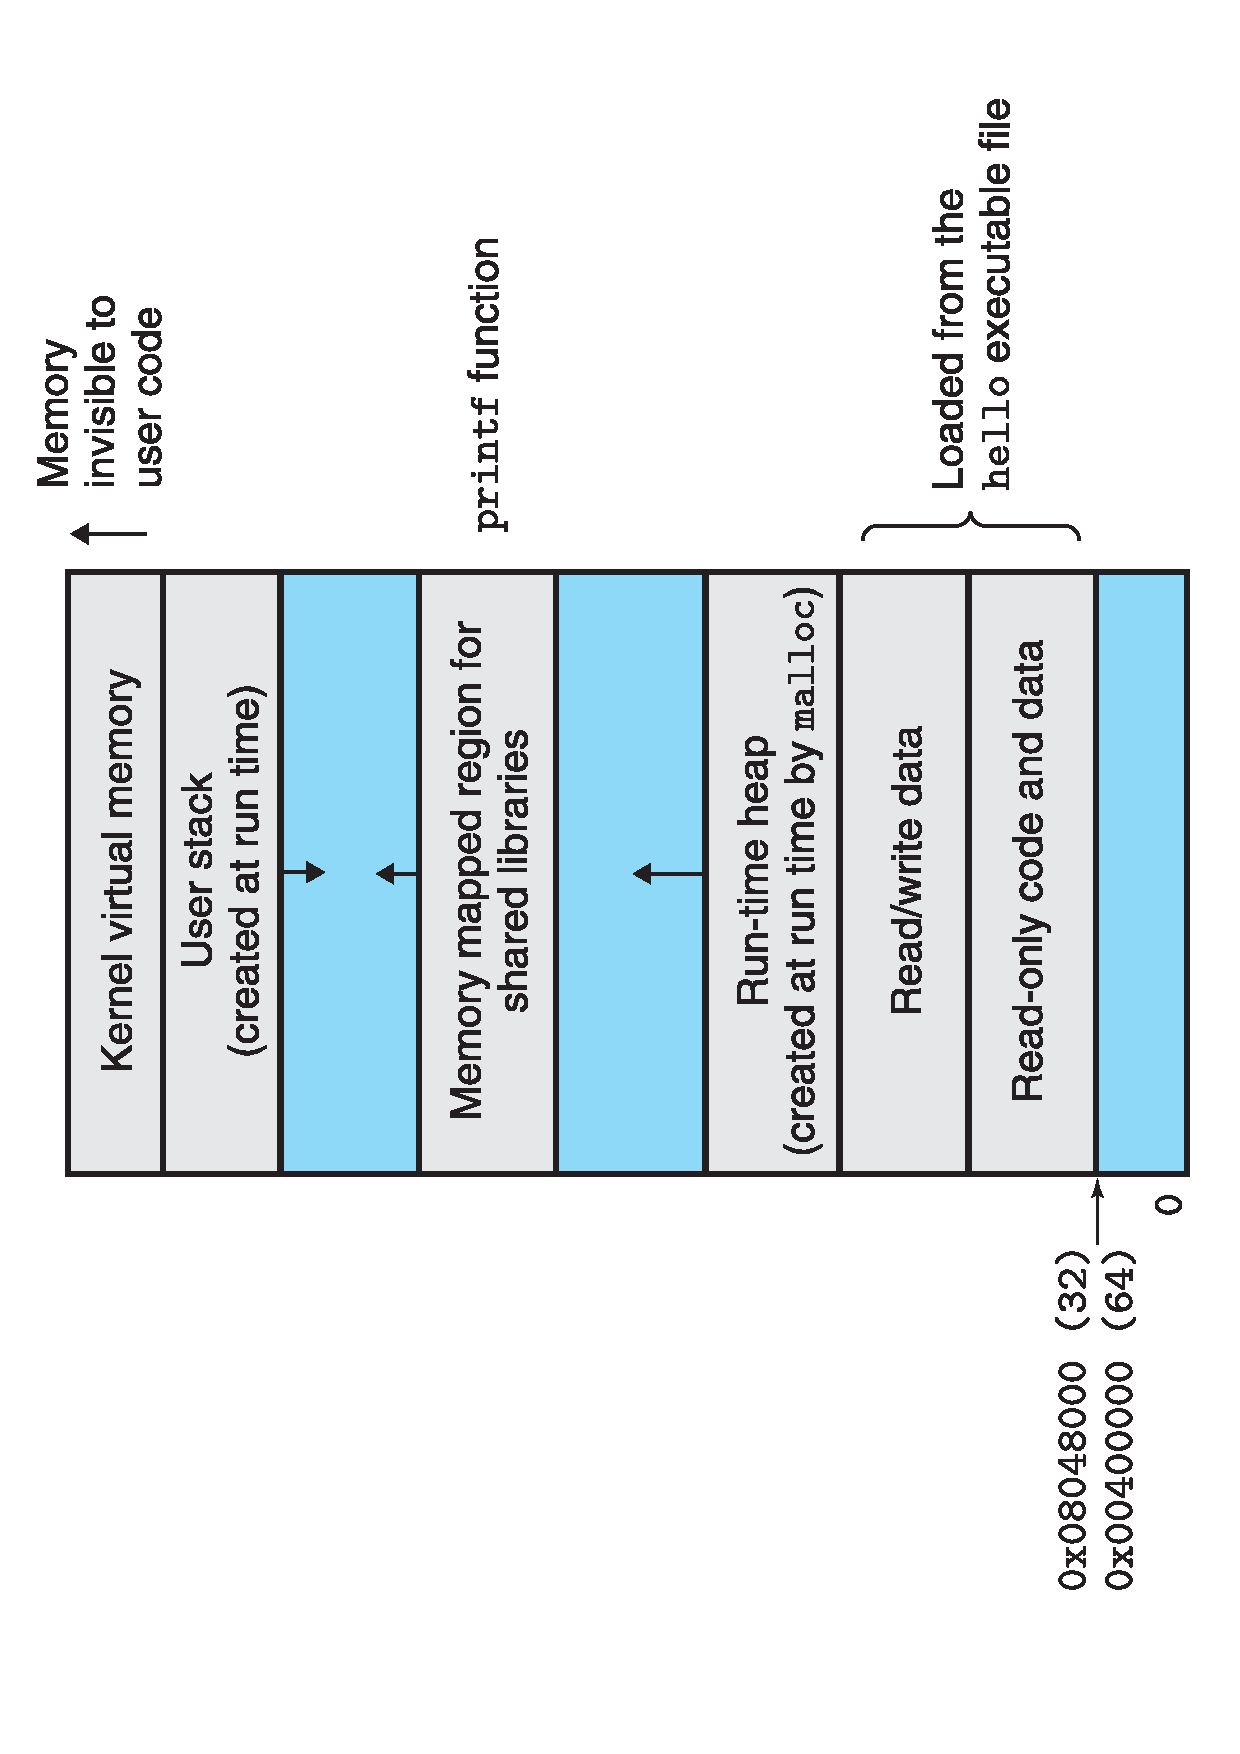
\includegraphics[keepaspectratio,width=0.5\paperwidth,angle=270]{Pictures/Kernel/process-mem-csapp.pdf}
	\caption{进程的典型内存布局示例}
	\label{fig:processmemlayout-csapp}
	\end{center}
\end{figure}

图 \ref{fig:processmemlayout-csdn}是从CSDN上找到的:
\begin{figure}[ht]
	\begin{center}
		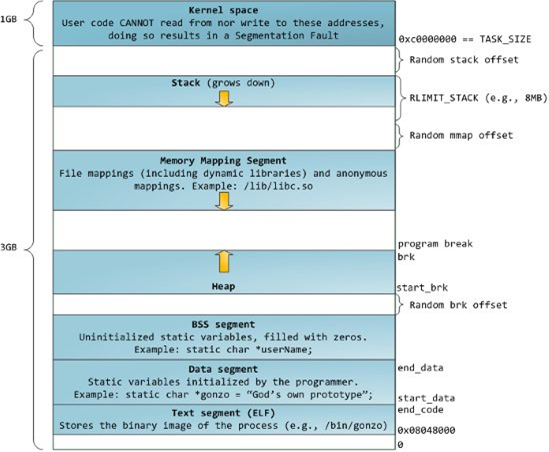
\includegraphics[keepaspectratio,width=0.5\paperwidth]{Pictures/Kernel/LinuxCppMemLayout3.png}
	\caption{进程的典型内存布局示例}
	\label{fig:processmemlayout-csdn}
	\end{center}
\end{figure}


最高地址区域又叫内核虚拟存储器,是用户代码不可见区域。
ESP指向栈顶,通过brk/sbrk系统调用扩大堆,向上增长。
小于0x0804 8000为保留区域,进而是只读段。
在glibc实现的内存管理算法中,Malloc小块内存是在小于0x4000 0000的内存中分配的,通过brk/sbrk不断向上扩展,而分配大块内存,malloc直接通过系统调用mmap实现,分配得到的地址在文件映射区,所以其地址大于0x4000 0000。
值得注意的是,字符串字面值(如"Hello World")存储在代码段(只读段)。

图\ref{fig:processmemlayout-csapp}所描述的模型无法适用于多线程环境。
按图\ref{fig:processmemlayout-csapp}所述,程序最多拥有上GB的栈空间,事实上,在多线程情况下,能用的栈空间是非常有限的, 可能只有几MB,超这个范围就会造成栈溢出。
线程的堆栈一般都是在线程创建的时候就固定分配好了的,线程切换的时候需要保存的是栈顶指针。
Windows线程的缺省堆栈大小为1M,Linux默认8M。

同一个进程中的多个线程,它们的内存空间是共享的(栈除外),在一个线程修改的内存内容,对所有线程都生效。这是一个优点也是一个缺点。说它是优点,线程的数据交换变得非常快捷。说它是缺点,一个线程死掉了,其它线程也性命不保; 多个线程访问共享数据,需要昂贵的同步开销,也容易造成同步相关的BUG。

线程间共享:地址空间,全局变量,打开文件,子进程,即将发生的报警,信号与信号处理程序,账户信息。线程私有:\textbf{程序计数器,寄存器,堆栈,状态}。
和传统进程一样(即只有一个线程的进程),线程可以处于若干种状态的任何一个:运行、阻塞、就绪或终止。 
线程自己的堆栈往往属于进程堆栈的一部分,thread switch时通常无需专门进行保存。thread switch时,往往只需要保存寄存器信息,故switch的开销较小。

\subsection{Linux进程结构}
files\_struct结构保存了进程打开的所有文件表数据,描述一个正被打开的文件。

struct file文件结构体代表一个打开的文件,系统中的每个打开的文件在内核空间都有一个关联的struct file。它由内核在打开文件时创建,并传递给在文件上进行操作的任何函数。在文件的所有实例都关闭后,内核释放这个数据结构。在内核创建和驱动源码中,struct file的指针通常被命名为file或filp。struct file包含的struct file\_operations成员包含着与文件关联的操作,如seek,read,write。

\begin{figure}[ht]
	\begin{center}
		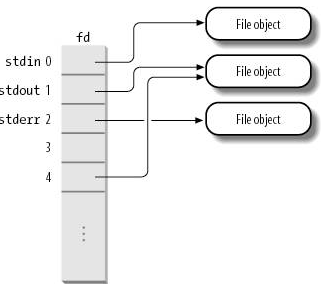
\includegraphics[keepaspectratio,width=0.3\paperwidth]{Pictures/Kernel/LinuxFdArrayInFileStruct.png}
	\caption{file\_struct中的fd数组}
	\label{fig:LinuxFdArrayInFileStruct}
	\end{center}
\end{figure}

\begin{figure}[ht]
	\begin{center}
		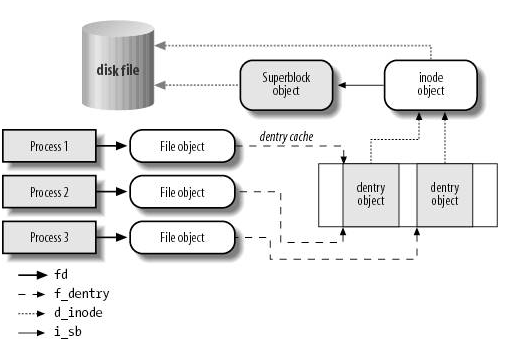
\includegraphics[keepaspectratio,width=0.4\paperwidth]{Pictures/Kernel/LinuxProcessAndVFS.png}
	\caption{进程与VFS的交互}
	\label{fig:LinuxProcessAndVFS}
	\end{center}
\end{figure}

\subsection{Linux线程模型}

线程的实现分为两种方式,多对一模型和一对一模型。
多对一模型下,内核对线程无知,以进程为调度单位,而线程调度是由用户进程完成的,可理解成进程将内核分配给自己的时间片二次分配给自己的线程。
此设计缺点明显:线程的阻塞导致进程阻塞。
一对一模型下,内核以线程为单位进行调度,LinuxThreads和NPTL均使用一对一模型。

LinuxThread使用clone系统调用来产生“线程”,这里的线程虽符合轻量进程的定义, 但它又具备了进程的若干特性,如拥有独立的进程id和信号机制等等。
内核在进行调度时,仍然按照传统的进程调度机制,在这个意义上,是将“线程”当作进程来处理的,内核对线程并无特殊支持。

 LinuxThreads 设计的一些局限性:
 \begin{itemize}
 \item 由于它是围绕一个管理线程来设计的,因此会导致很多的上下文切换的开销,这可能会妨碍系统的可伸缩性和性能。
 由于管理线程只能在一个 CPU 上运行,因此所执行的同步操作在 SMP 或 NUMA 系统上可能会产生可伸缩性的问题。
 \item 由于线程的管理方式,以及每个线程都使用了一个不同的进程 ID,对信号的处理是按照每线程的原则建立的, 因此 LinuxThreads 与其他与 POSIX 相关的线程库并不兼容。
 \item 由于内核实际上将线程“认作”进程,因此针对进程的诸多限制也被应用在线程上,比如可用进程总数等, /proc下也有大量进程项对应线程。
 \end{itemize}

NPTL,或称为 Native POSIX Thread Library,是 Linux 线程的一个新实现,它克服了 LinuxThreads 的缺点,同时也符合 POSIX 的需求。
与 LinuxThreads 相比,它在性能和稳定性方面都提供了重大的改进。自2.6内核以来,NPTL取代LinuxThreads成为了新的Linux线程标准。

NPTL使用了跟LinuxThread相同的办法,在内核里面线程仍然被当作是一个进程,并且仍然使用了clone()系统调用(在NPTL库里调用)。
但是,NPTL需要内核级的特殊支持来实现,比如需要挂起然后再唤醒线程的线程同步原语futex。

与 LinuxThreads 相比,NPTL 具有很多优点: NPTL没有使用管理线程。
管理线程的一些需求,例如向作为进程一部分的所有线程发送终止信号,是并不需要的;因为内核本身就可以实现这些功能。
内核还会处理每个线程堆栈所使用的内存的回收工作。它甚至还通过在清除父线程之前进行等待,从而实现对所有线程结束的管理,这样可以避免僵尸进程的问题。
由于 NPTL 没有使用管理线程,因此其线程模型在 NUMA 和 SMP 系统上具有更好的可伸缩性和同步机制。

\subsection{Thread-local storage}
Thread-local storage (TLS) 指“局部”于线程的静态/全局地址位置,实际上是说当多个线程引用同一静态/全局变量时,实际上是引用了不同的地址位置。

Windows API和Pthread均提供了操纵TLS变量的接口。C++11 引人了thread\_local 关键词,定义TLS变量,此外,gcc使用如\verb$__thread int number;$语法定义TLS。
Python如此使用TLS:

\begin{lstlisting}[language=Python]
import threading
mydata = threading.local()
mydata.x = 1
\end{lstlisting}

\subsection{进程同步}
进程同步是一个操作系统级别的概念,是在多道程序的环境下,存在着不同的制约关系,为了协调这种互相制约的关系,实现资源共享和进程协作,从而避免进程之间的冲突,引入了进程同步。

进程同步的机制有:
\begin{itemize}
\item 信号量
\item 自旋锁
\item 原子操作
\item 管程
\item 会和
\item 分布式系统
\end{itemize}

管程 (英语:Moniters,也称为监视器) 是一种程序结构,结构内的多个子程序(对象或模块)形成的多个工作线程互斥访问共享资源。这些共享资源一般是硬件设备或一群变量。管程实现了在一个时间点,最多只有一个线程在执行管程的某个子程序。与那些通过修改数据结构实现互斥访问的并发程序设计相比,管程实现很大程度上简化了程序设计。
管程提供了一种机制,线程可以临时放弃互斥访问,等待某些条件得到满足后,重新获得执行权恢复它的互斥访问。
东尼·霍尔证明了这与信号量是等价的。在编程语言Concurrent Pascal,Pascal-Plus,Modula-2,Modula-3,Mesa以及Java中都提供这个功能。

一个管程包含:多个彼此可以交互并共用资源的线程,多个与资源使用有关的变量,一个互斥锁,一个用来避免竞态条件的不变量。
一个管程的程序在运行一个线程前会先取得互斥锁,直到完成线程或是线程等待某个条件被满足才会放弃互斥锁。若每个执行中的线程在放弃互斥锁之前都能保证不变量成立,则所有线程皆不会导致竞态条件成立。

当一个线程执行管程中的一个子程序时,称为占用(occupy)该管程. 管程的实现确保了在一个时间点,最多只有一个线程占用了该管程。这是管程的互斥锁访问性质。

\subsection{僵尸进程}
在UNIX 系统中,一个进程结束了,但是他的父进程没有等待(调用wait/waitpid)他, 那么他将变成一个\textbf{僵尸进程}。
系统调用exit,它的作用是使进程退出,但也仅仅限于将一个正常的进程变成一个僵尸进程,并不能将其完全销毁。
即使是root身份kill-9也不能杀死僵尸进程。
补救办法是杀死僵尸进程的父进程(僵尸进程的父进程必然存在),僵尸进程成为"孤儿进程",过继给1号进程init,init始终会负责清理僵尸进程。
在Linux进程的状态中,僵尸进程是非常特殊的一种,它已经放弃了几乎所有内存空间,没有任何可执行代码,也不能被调度,仅仅在进程列表中保留一个位置,
记载该进程的退出状态等信息供其他进程收集,除此之外,僵尸进程不再占有任何内存空间。
僵尸进程占用了进程号资源,同时记录着进程的退出状态、进程运行的CPU时间等。

为避免僵尸进程,父进程可以用signal函数为SIGCHLD安装handler,因为子进程结束后, 父进程会收到该信号,可以在handler中调用wait回收;
也可以用signal(SIGCHLD,SIG\_IGN) 通知内核,自己对子进程的结束不感兴趣,那么子进程结束后,内核会回收,并不再给父进程发送信号。

\subsection{进程通信}
共享存储系统、消息传递系统、管道(以文件系统为基础)。

信号的处理方式包括:忽略,捕捉(调用用户函数),执行默认动作。
有两种信号不能忽略:SIGKILL,SIGSTOP。它们向超级用户提供了使进程终止或停止的可靠方法。

\subsection{协程与线程的区别}
1. 协程并非os线程,所以创建、切换开销比线程相对要小。
        2. 协程与线程一样有自己的栈、局部变量等,但是协程的栈是在用户进程空间模拟的,所以创建、切换开销很小。
        3. 多线程程序是多个线程并发执行,也就是说在一瞬间有多个控制流在执行。而协程强调的是一种多个协程间协作的关系,只有当一个协程主动放弃执行权,另一个协程才能获得执行权,所以在某一瞬间,多个协程间只有一个在运行。
        4. 由于多个协程时只有一个在运行,所以对于临界区的访问不需要加锁,而多线程的情况则必须加锁。
        5. 多线程程序由于有多个控制流,所以程序的行为不可控,而多个协程的执行是由开发者定义的所以是可控的。


\clearpage

















%!Mode:: "TeX:UTF-8"
\section{栈溢出和堆溢出}

A thread's assigned stack size can be as small as a few dozen kilobytes. Allocating more memory on the stack than is available can result in a crash due to stack overflow.

\begin{figure}[ht]
	\begin{center}
		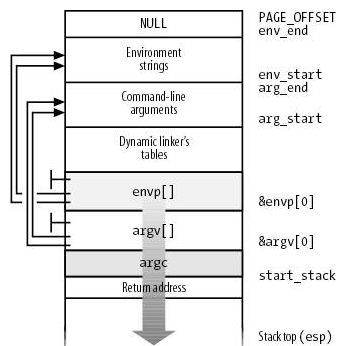
\includegraphics[keepaspectratio,width=0.3\paperwidth]{Pictures/LinuxUserStack.png}
	\caption{用户栈顶端}
	\label{fig:LinuxUserStack}
	\end{center}
\end{figure}

栈和堆溢出的一个共性就是第三方可以完全依靠提供特定数据实现代码级别的入侵。
堆溢出执行恶意代码的一种情况是通过过长的数据破坏堆管理记录结构,使下次申请能得到保存某些特定函数指针的位置,然后进行修改。
此外,由于字符串处理函数(gets,strcpy等等)没有对数组越界加以监视和限制,我们利用字符数组写越界,覆盖堆栈中的老元素的值,就可以修改返回地址。 

gets函数(\verb$char *gets(char *s);$)和fgets(\verb$char *fgets(char*, int, FILE*);$)函数最大的不同是gets函数的缓冲区虽然由用户提供,但是用户无法指定其一次最多读入多少字节的内容。这一点导致gets变成了一个非常危险的函数。

有时,堆和栈的溢出分别指内存空间的耗尽。
递归可能会导致栈耗尽,内存泄露会导致堆耗尽。
 
\clearpage
%!Mode:: "TeX:UTF-8"
\section{Linux启动过程}


\subsection{BIOS}
BIOS是英文"Basic Input Output System"的缩略语,它是一组固化到计算机内主板上一个ROM芯片上的程序,它保存着计算机最重要的基本输入输出的程序、系统设置信息、开机后自检程序和系统自启动程序。 其主要功能是为计算机提供最底层的、最直接的硬件设置和控制。

\textbf{Bootloader即引导装入程序},是由BIOS用来把操作系统内核镜像装载到RAM中所调用的一个程序。
它在系统上电时开始执行,初始化硬件设备、准备好软件环境,最后调用系统内核。
Linux在x86下的引导装入程序有Linux Loader(LILO)和GRUB,GRUB更高级,本文假定使用LILO。

硬盘的第一个扇区称为MBR(Master Boot Record),该扇区包含一个分区表和一个小程序,这个小程序用来装载被启动的操作系统所在分区的第一个扇区。Windows 98使用分区表中的active标志来标示活动分区,只有内核镜像存在活动分区中的操作系统才可被启动。而Linux的处理方式更为灵活,用一个Bootloader取代这个MBR中不完善的程序,允许用户来选择要启动的操作系统。
LILO或许在MBR上,取代了那个小程序,或许被装在每个分区的引导扇区上。

用户选择引导Linux后,LILO调用BIOS例程打印“Loading”信息,从磁盘读取内核镜像。
\verb$setup()$函数的代码在内核镜像文件的0x200处,LILO装载完内核镜像后会跳转到\verb$setup()$函数处。
\verb$setup()$最终跳转到\verb$startup_32()$函数处。

\verb$startup_32()$函数有两个,依次执行。
其中第二个\verb$startup_32()$会创建被称作进程0的内核线程(又称\textbf{idle进程或swapper进程})。进程0是内核的一部分,不执行任何磁盘程序。
进程0调用\verb$start_kernel()$。

\verb$start_kernel()$初始化内核所需的所有数据结构(此前只有少数几个数据结构被建立),激活中断,创建一个叫进程1的内核线程,又叫\textbf{init进程}。
init进程执行\verb$init()$函数,\verb$init()$完成内核初始化。\verb$init()$函数调用\verb$execve()$装入可执行程序init,结果
init内核线程变成了一个普通进程,并拥有了自己的per-process内核数据结构。在系统关闭前,init进程一直存活,因为它创建和监控在操作系统外层执行的所有进程的活动。

\subsection{init进程}

系统加电之后,首先进行的硬件自检,然后是bootloader对系统的初始化,加载内核。
内核被加载到内存中之后,就开始执行了。
一旦内核启动运行,对硬件的检测就会决定需要对哪些设备驱动程序进行初始化。
从这里开始,内核就能够挂装根文件系统。
内核挂装了根文件系统,并已初始化所有的设备驱动程序和数据结构等之后,就通过启动一个叫init的用户级程序,完成引导进程。

由0号进程创建1号进程(内核态),1号负责执行内核的部分初始化工作及进行系统配置,并创建若干个用于高速缓存和虚拟主存管理的内核线程。随后,1号进程调用execve()运行可执行程序init,并演变成用户态1号进程,即init进程。它按照配置文件/etc/initab的要求,完成系统启动工作,创建编号为1号、2号...的若干终端注册进程getty。每个getty进程设置其进程组标识号,并监视配置到系统终端的接口线路。当检测到来自终端的连接信号时,getty进程将通过函数\verb$execve()$执行注册程序login,此时用户就可输入注册名和密码进入登录过程,如果成功,由login程序再通过函数\verb$execve()$执行shell,该shell进程接收getty进程的pid,取代原来的getty进程。再由shell直接或间接地产生其他进程。

上述过程可描述为:0号进程->1号内核进程->1号内核线程->1号用户进程(init进程)->getty进程->shell进程。


\subsection{init程序}

init是 Unix 和 类Unix 系统中用来产生其它所有进程的程序。它以守护进程的方式存在,其进程号为1。

BSD init 运行存放于'/etc/rc'的初始化 shell 脚本,然后启动基于文本模式的终端(getty)或者基于图形界面的终端(窗口系统,如 X)。
这里没有运行模式的问题,因为文件 'rc' 决定了 init 如何执行。

现代的 BSD 派生系统一直支持使用 'rc.local'
文件的方式,它将在正常启动过程接近最后的时间以子脚本的方式来执行。这样做减少了整个系统无法启动的风险。然后,第三方软件包可以将它们独立的 start/stop 脚本安装到一个本地的 'rc.d' 目录中(通常这是由 ports collection/pkgsrc 完成的)。 FreeBSD 和 NetBSD 现在默认使用 rc.d ,该目录中所有的用户启动脚本,都被分成更小的子脚本,和 SysV 类似。

System V init 检查 '/etc/inittab' 文件中是否含有 'initdefault' 项。 这告诉 init
系统是否有一个默认运行模式。如果没有默认的运行模式,那么用户将进入系统控制台,手动决定进入何种运行模式。

systemd意欲取代System V和BSD风格的init的程序。
在RHEL6中采用的init程序为upstart。在RHEL7中开始采用systemd。

   
\subsection{运行级别}
\begin{itemize}
  \item 0为停机,机器关闭。 
  \item 1为单用户模式,就像Win9x下的安全模式类似。 
  \item 2为多用户模式,但是没有NFS支持。 
  \item 3为完整的多用户模式,是标准的运行级。除了需要在登录后手动启动图形界面外,与级别5相同。
  \item 4一般的发行版没定义这个级别。
  \item 5就是X11,进到X Window系统了。 
  \item 6为重启,运行init 6机器就会重启。 
\end{itemize}
在Ubuntu 14.04上尝试进入级别2,3,4,5均处于X11界面,进入级别1系统退出并卡死。

查看运行级别命令:
 \begin{verbatim}
 runlevel
\end{verbatim}
先后显示系统上一次和当前运行级别。如果不存在上一次运行级别,则用N表示。在Ubuntu上运行结果为“N 2”。

改变提供运行级别命令:
 \begin{verbatim}
 init [0123456]
\end{verbatim}


    
\subsection{内核线程}
除了idle和init进程之外,其他内核线程包括:
\begin{description}
  \item[keventd] 执行\verb$kevent_wq$工作队列中的函数。
  \item[kapmd] 处理与APM(高级电源管理)相关的事件。
  \item[kswapd] 执行内存回收。
  \item[pdflush] 刷新脏内存的内容到磁盘以回收内存。
  \item[kblockd] 执行\verb$kblockd_workqueue$工作队列中的函数。它周期性激活块设备驱动程序, 因为一些需要激活驱动程序的work已被延迟以求提高性能。
  \item[ksoftirqd] 每个CPU都有一个ksoftirqd,运行tasklet。
\end{description}




















    
    
    
    
    
    
    
    
    
    
    
    
    

%!Mode:: "TeX:UTF-8"
\section{死锁}


死锁产生的现场:当A进程P S2信号量而B进程P S1信号量时就会产生死锁,因为S2信号量需要B进程释放,而S1信号量需要A进程释放,因此两个进程都在等相互的资源,造成死锁。

\begin{figure}[ht]
	\begin{center}
		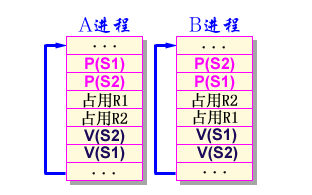
\includegraphics[keepaspectratio,width=0.5\paperwidth]{Pictures/deadlock.png}
	\caption{死锁示例}
	\label{fig:deadlock}
	\end{center}
\end{figure}

死锁产生的条件:
\begin{itemize}
\item  
互斥条件:进程要求对所分配的资源进行排它性控制,即在一段时间内某资源仅为一进程所占用。(信号量s1 s2为互斥的信号量,只能被一个进程占用)
\item  
请求和保持(部分分配,占有申请):已持有资源的进程可以请求新资源(A进程在获取s2阻塞时,一直占用s1)
\item  
不可剥夺条件:进程已获得的资源在未使用完之前,不能剥夺,只能在使用完时由自己释放。(s1只能由A进程释放,s2只能由B进程释放)
\item  
环路等待条件:在发生死锁时,必然存在一个进程--资源的环形链。(A B 进程都是环形链路)
\end{itemize}

为避免死锁,可以从上述后三个条件入手,而第一个互斥条件是无法被破坏的\cite{pibible}。

银行家算法(Banker's Algorithm)是一个避免死锁(Deadlock)的著名算法,是由Edsger Dijkstra 在1965年为T.H.E系统设计的一种避免死锁产生的算法。它以银行借贷系统的分配策略为基础,判断并保证系统的安全运行。

如果所有过程有可能完成执行(终止),则一个状态(如上述范例)被认为是安全的。由于系统无法知道什么时候一个过程将终止,或者之后它需要多少资源,系统假定所有进程将最终试图获取其声明的最大资源并在不久之后终止。在大多数情况下,这是一个合理的假设,因为系统不是特别关注每个进程运行了多久(至少不是从避免死锁的角度)。此外,如果一个进程终止前没有获取其它能获取的最多的资源,它只是让系统更容易处理。


基于这一假设,该算法通过尝试寻找允许每个进程获得的最大资源并结束(把资源返还给系统)的进程请求的一个理想集合,来决定一个状态是否是安全的。不存在这个集合的状态都是不安全的。如果一个资源请求无法被满足,则驳回。如果该请求key被满足,但导致系统离开了安全状态,则该请求不被受理,即延缓执行或驳回。

%!Mode:: "TeX:UTF-8"
 
\section{外设}


\begin{figure}[ht]
	\begin{center}
		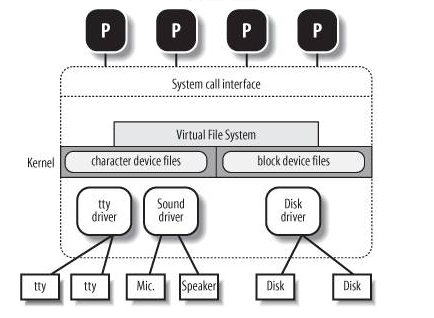
\includegraphics[keepaspectratio,width=0.5\paperwidth]{Pictures/Kernel/LinuxDriverInf.png}
	\caption{Linux外设接口模型}
	\label{fig:LinuxDriverInf}
	\end{center}
\end{figure}

\begin{figure}[ht]
	\begin{center}
		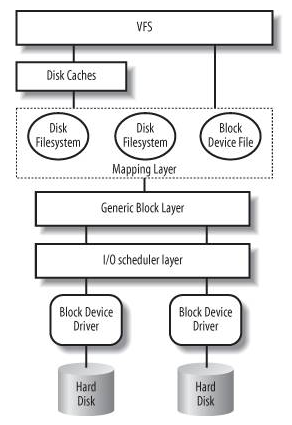
\includegraphics[keepaspectratio,width=0.4\paperwidth]{Pictures/Kernel/kernelComponentForBlockDeviceOp.png}
	\caption{与块设备操作相关的内核组件}
	\label{fig:kernelComponentForBlockDeviceOp}
	\end{center}
\end{figure}

在对块设备进行I/O操作时,图 \ref{fig:kernelComponentForBlockDeviceOp}中的映射层将”文件偏移量,读写长度“数值对映射为若干组连续的磁盘逻辑块,必要时借助文件系统(读取inode)。
通用块层对每组连续的块发起BIO操作。
内核中用inode结构表示索引节点,可以是文件,也可以是目录。inode(可理解为ext2 inode)对应于物理磁盘上的具体对象。


\begin{figure}[ht]
	\begin{center}
		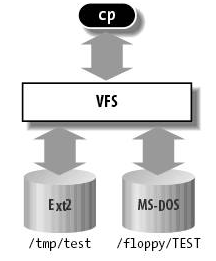
\includegraphics[keepaspectratio,width=0.15\paperwidth]{Pictures/Kernel/VirtualFileSystem.png}
	\caption{VFS在copy操作中的作用}
	\label{fig:VirtualFileSystem}
	\end{center}
\end{figure}


\begin{figure}[ht]
	\begin{center}
		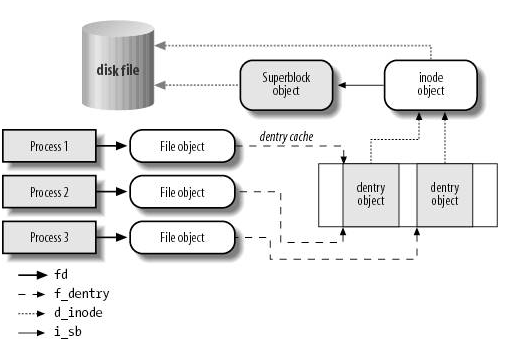
\includegraphics[keepaspectratio,width=0.4\paperwidth]{Pictures/Kernel/LinuxProcessAndVFS.png}
	\caption{进程与VFS的交互}
	\label{fig:LinuxProcessAndVFS}
	\end{center}
\end{figure}

\begin{figure}[ht]
	\begin{center}
		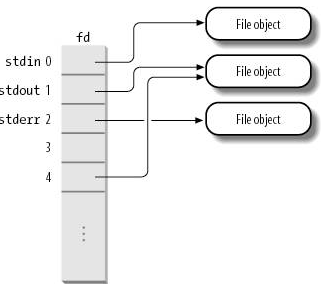
\includegraphics[keepaspectratio,width=0.3\paperwidth]{Pictures/Kernel/LinuxFdArrayInFileStruct.png}
	\caption{file\_struct中的fd数组}
	\label{fig:LinuxFdArrayInFileStruct}
	\end{center}
\end{figure}


\begin{figure}[ht]
	\begin{center}
		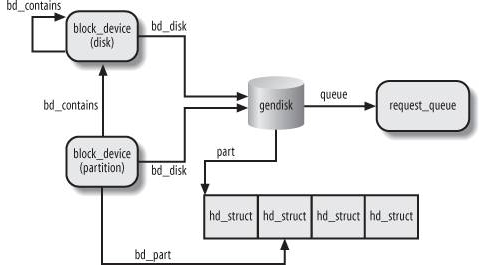
\includegraphics[keepaspectratio,width=0.6\paperwidth]{Pictures/Kernel/BlockDeviceDescriptors.png}
	\caption{块设备描述符}
	\label{fig:BlockDeviceDescriptors}
	\end{center}
\end{figure}













\clearpage


%!Mode:: "TeX:UTF-8"
\section{分布式系统}

分布式计算技术是一门计算机科学,它研究如何把一个需要非常巨大的计算能力才能解决的问题分成许多小的部分,然后把这些部分分配给许多计算机进行处理,最后把这些计算结果综合起来得到最终的结果。
共享稀有资源和平衡负载是计算机分布式计算的核心思想之一。

在一个分布式系统中,一组独立的计算机展现给用户的是一个统一的整体,就好像是一个系统似的。系统拥有多种通用的物理和逻辑资源,可以动态的分配任务,分散的物理和逻辑资源通过计算机网络实现信息交换。系统中存在一个以全局的方式管理计算机资源的分布式操作系统。通常,对用户来说,分布式系统只有一个模型或范型。在操作系统之上有一层软件中间件(middleware)负责实现这个模型。一个著名的分布式系统的例子是万维网(World Wide Web),在万维网中,所有的一切看起来就好像是一个文档(Web页面)一样。

分布式软件系统(Distributed Software Systems)是支持分布式处理的软件系统,是在由通信网络互联的多处理机体系结构上执行任务的系统。它包括分布式操作系统、分布式程序设计语言及其编译(解释)系统、分布式文件系统和分布式数据库系统等。

\subsection{CORBA}
CORBA (Common Object Request Broker Architecture) 是在1992年由OMG(Open Management Group) 组织提出的软件构建标准。
那时的分布式应用环境都采用Client/Server架构,CORBA的应用很大程度的提高了分布式应用软件的开发效率。

\subsection{DCOM}
当时的另一种分布式系统开发工具是Microsoft的DCOM(Distributed Common Object Model)。Microsoft为了使在Windows平台上开发的各种应用软件产品的功能能够在运行时(Runtime)相互调用(比如在Microsoft Word中直接编辑Excel文件),实现了OLE(Linked and Embedded Object)技术,后来这个技术衍生为COM(Common Object Model)。

\subsection{J2EE}
随着Internet的普及和网络服务(Web Services)的广泛应用, Browser/Server架构的模式逐渐体现出它的优势。 于是,Sun公司在其Java技术的基础上推出了应用于B/S架构的J2EE的开发和应用平台;Microsoft也在其DCOM技术的基础上推出了主要面向B/S应用的.NET开发和应用平台。

J2EE是一套全然不同于传统应用开发的技术架构,包含许多组件,主要可简化且规范应用系统的开发与部署,进而提高可移植性、安全与再用价值。

J2EE核心是一组技术规范与指南,其中所包含的各类组件、服务架构及技术层次,均有共同的标准及规格,让各种依循J2EE架构的不同平台之间,存在良好的兼容性,解决过去企业后端使用的信息产品彼此之间无法兼容,企业内部或外部难以互通的窘境。

J2EE组件和“标准的” Java类的不同点在于:它被装配在一个J2EE应用中,具有固定的格式并遵守J2EE规范,由J2EE服务器对其进行管理。J2EE规范是这样定义J2EE组件的:客户端应用程序和applet是运行在客户端的组件;Java Servlet和Java Server Pages (JSP) 是运行在服务器端的Web组件;Enterprise Java Bean (E JB )组件是运行在服务器端的业务组件。

\subsection{Hadoop}
Hadoop是一个分布式系统基础架构,由Apache基金会所开发。用户可以在不了解分布式底层细节的情况下,开发分布式程序。充分利用集群的威力进行高速运算和存储。
Hadoop实现了一个分布式文件系统(Hadoop Distributed File System),简称HDFS。HDFS有高容错性的特点,并且设计用来部署在低廉的(low-cost)硬件上;而且它提供高吞吐量(high throughput)来访问应用程序的数据,适合那些有着超大数据集(large data set)的应用程序。HDFS放宽了(relax)POSIX的要求,可以以流的形式访问(streaming access)文件系统中的数据。
Hadoop的框架最核心的设计就是:HDFS和MapReduce。HDFS为海量的数据提供了存储,则MapReduce为海量的数据提供了计算。






%!Mode:: "TeX:UTF-8"
\section{调度}

\subsection{作业调度}
作业调度,也称批处理,简称 BP(batch processing),是指在计算机上无须人工干预而执行系列程序的作业。
批处理任务无须人工交互,所有的输入数据预先设置于程序或命令行参数中。这是不同于需要用户输入数据的交互程序的概念。
批处理的发展远胜当初的大型电脑上的应用,现在也常用于UNIX环境,用CRON和at机制来安排复杂的工作程序。微软的DOS和Windows系统也有类似的命令描述语言,称为批处理文件。
批处理是相对于实时处理,在公共交通中,公共小巴时常都是用批处理的方法运输乘客的。
办公室内的激光打印机,也是以批处理的方法,应付多于一个客端用户的打印指令,避免打印输出混乱。

Shortest job next (SJN), 又称 Shortest Job First (SJF) 或 Shortest Process Next (SPN), 选择具有最短执行时间的作业来执行,为非抢占式调度算法,
而 Shortest remaining time 为其抢占式变种。

\textbf{Generalized processor sharing (GPS)} is a service policy for multiple classes of customers where service capacity is shared between customer classes according to some fixed weights. Service is shared between all non-empty classes in the same ratio as the weight factors (positive values for each service class). In processor scheduling, generalized processor sharing is "an idealized scheduling algorithm that achieves perfect fairness. All practical schedulers approximate GPS and use it as a reference to measure fairness."Generalized processor sharing assumes that traffic is fluid (infinitesimal packet sizes), and can be arbitrarily split. There are several service disciplines which track the performance of GPS quite closely such as weighted fair queuing (WFQ)[4] and known as packet-by-packet generalized processor sharing (PGPS).

\textbf{Weighted round robin (WRR)} is a scheduling discipline. Each packet flow or connection has its own packet queue in a network interface card. It is the simplest approximation of generalized processor sharing (GPS). While GPS serves infinitesimal amounts of data from each nonempty queue, WRR serves a number of packets for each nonempty queue.

速率单调(RM)算法是C. L. LIU(刘炯朗)和J. W. LAYLAND提出的单处理机实时周期性任务静态优先级调度算法。
该算法的按照任务的速率分配优先级。速率越大,优先级越高;速率越小,优先级越低。
These operating systems are generally preemptive and have deterministic guarantees with regard to response times. Rate monotonic analysis is used in conjunction with those systems to provide scheduling guarantees for a particular application.

\textbf{Highest Response Ratio Next (HRRN)} scheduling is a non-preemptive discipline, similar to Shortest Job Next (SJN), in which the priority of each job is dependent on its estimated run time, and also the amount of time it has spent waiting. Jobs gain higher priority the longer they wait, which prevents indefinite postponement (process starvation). In fact, the jobs that have spent a long time waiting compete against those estimated to have short run times.
\begin{equation}
\mathrm{priority}=\frac{\mathrm{waitingTime}}{\mathrm{estimated Running Time}} + 1
\end{equation}

基于优先数调度算法(HPF):每一个作业规定一个表示该作业优先级别的整数,当需要将新的作业由输入井调入内存处理时,优先选择优先数最高的作业。


\subsection{I/O调度}
Linux的I/O调度算法又称电梯算法,主要有:
\begin{description}
    \item[CFQ(完全公平排队)] 在最新的内核版本和发行版中,都选择CFQ做为默认的I/O调度器,对于通用的服务器也是最好的选择。	CFQ实现了一种QoS的IO调度算法。该算法为每一个进程分配一个时间窗口,在该时间窗口内,允许进程发出IO请求。通过时间窗口在不同进程间的移动,保证了对于所有进程而言都有公平的发出IO请求的机会。同时CFQ也实现了进程的优先级控制,可保证高优先级进程可以获得更长的时间窗口。
	CFQ为每个进程/线程,单独创建一个队列来管理该进程所产生的请求,也就是说每个进程一个队列,各队列之间的调度使用时间片来调度。
    \item[NOOP] NOOP调度器十分简单,其只拥有一个等待队列,每当来一个新的请求,仅仅是按先来先处理的思路将请求插入到等待队列的尾部。
其应用环境主要有以下两种:一是物理设备中包含了自己的I/O调度程序,比如SCSI的TCQ;二是寻道时间可以忽略不计的设备,比如SSD等。
    \item[Deadline(截止时间调度程序)] DEADLINE调度算法主要针对I/O请求的延时而设计,每个I/O请求都被附加一个最后执行期限。
	该算法维护两类队列,一是按照扇区排序的读写请求队列;二是按照过期时间排序的读写请求队列。
	如果当前没有I/O请求过期,则会按照扇区顺序执行I/O请求;
	如果发现过期的I/O请求,则会处理按照过期时间排序的队列,直到所有过期请求都被发射为止。
	在处理请求时,该算法会优先考虑读请求。
	当系统中存在的I/O请求进程数量比较少时,与CFQ算法相比,DEADLINE算法可以提供较高的I/O吞吐率。
\item[AS(预料I/O调度程序)]CFQ和DEADLINE考虑的焦点在于满足零散IO请求上。对于连续的IO请求,比如顺序读,并没有做优化。为了满足随机IO和顺序IO混合的场 景,Linux还支持ANTICIPATORY调度算法。ANTICIPATORY的在DEADLINE的基础上,为每个读IO都设置了6ms的等待时间 窗口。如果在这6ms内OS收到了相邻位置的读IO请求,就可以立即满足。
\end{description}

在传统的SAS盘上,CFQ、DEADLINE、ANTICIPATORY都是不错的选择;对于专属的数据库服务器,DEADLINE的吞吐量和响应时间都表现良好。
然而在新兴的固态硬盘比如SSD、Fusion IO上,最简单的NOOP反而可能是最好的算法,因为其他三个算法的优化是基于缩短寻道时间的,而固态硬盘没有所谓的寻道时间且IO响应时间非常短。

查看当前系统支持的IO调度算法
\begin{verbatim}
[root@localhost ~]# dmesg | grep -i scheduler
io scheduler noop registered
io scheduler anticipatory registered
io scheduler deadline registered
io scheduler cfq registered (default)
\end{verbatim}


查看当前系统的I/O调度方法:
\begin{verbatim}
cat /sys/block/sda/queue/scheduler
noop anticipatory deadline [cfq]
\end{verbatim}


临地更改I/O调度方法:
\begin{verbatim}
echo noop > /sys/block/sda/queue/scheduler
\end{verbatim}


想永久的更改I/O调度方法,需修改内核引导参数,加入elevator=调度程序名
\begin{verbatim}
vi /boot/grub/menu.lst
更改到如下内容:
kernel /boot/vmlinuz-2.6.18-8.el5 ro root=LABEL=/ elevator=deadline rhgb quiet
\end{verbatim}


\subsection{进程调度}
参考\url{http://blog.csdn.net/zhoudaxia/article/details/7375668}

Ingo Molnar开发了O(1)调度器,在CFS和RSDL之前,这个调度器不仅被Linux2.6采用,还被backport到Linux2.4中,很多商业的发行版本都采用了这个调度器。
每个CPU都有两个进程队列,采用优先级为基础的调度策略。
内核为每个进程计算出一个反映其运行“资格”的权值,然后挑选权值最高的进程投入运行。在运行过程中,当前进程的资格随时间而递减,从而在下一次调度的时候原来资格较低的进程可能就有资格运行了。到所有进程的资格都为零时,就重新计算。
调度程序运行时,要在所有可运行的进程中选择最值得运行的进程。

选择进程的依据主要有task\_struct结构中有以下四项:
调度策略(policy, 取值有SCHED\_OTHER、SCHED\_FIFO 和 SCHED\_RR)、
静态优先级(priority)、
动态优先级(counter,进程剩余的时间片,它的起始值就是priority的值)、以及实时优先级(rt\_priority,实时进程特有的)。
在进程运行过程中,counter不断减少,而priority保持不变,以便在counter变为0的时候(该进程用完了所分配的时间片)对counter重新赋值。


对于实时进程,Linux采用了两种调度策略,即SCHED\_FIFO(先来先服务调度)和SCHED\_RR(时间片轮转调度)。
因为实时进程具有一定程度的紧迫性,所以衡量一个实时进程是否应该运行,Linux采用了一个比较固定的标准。
实时进程的counter只是用来表示该进程的剩余时间片,并不作为衡量它是否值得运行的标准。
SCHED\_FIFO进程会一直运行,直到I/O阻塞或者主动释放CPU,或者是CPU被另一个具有更高rt\_priority的实时进程抢先。
SCHED\_OTHER为普通进程,采用动态优先调度策略。只要系统中有一个实时进程在运行,则任何SCHED\_OTHER进程都不能在任何CPU运行。
 
从某种意义上讲,所有位于当前队列的任务都将被执行并且都将被移到“过期”队列之中(实时进程则例外,交互性强的进程也可能例外)。
当这种事情发生时,情况就会有所变化,队列就会被进行切换,原来的“过期”队列成为当前队列,而空的当前队列也就变成了过期队列。

schedule()函数是完成进程调度的主要函数,并完成进程切换的工作,
它在/kernel/sched.c 中的定义如下:
\begin{lstlisting}[language=C++]
{
  ...
      int idx;
      ...
      preempt_disable();//关闭内核抢占
      ...
      //快速定位优先级最高(值最小)的非空就绪进程链表,每个优先级对应位图上的一格
      idx = sched_find_first_bit(array -> bitmap);
      queue = array -> queue + idx;//
      next = list_entry(queue -> next, task_t, run_list);//
      ...
      prev = context_switch(rq, prev, next);//
      ...
}
\end{lstlisting}
Linux2.4 调度系统在所有就绪进程的时间片都耗完以后在调度器中一次性重新计算,其中重算是用for循环相当耗时。
Linux2.6为每个CPU保留 active和expired两个优先级数组,active 数组中包含了有剩余时间片的任务,expired数组中包含了所有用完时间片的任务。当一个任务的时间片用完了就会重新计算其时间片,并插入到expired队列中,当 active队列中所有进程用完时间片时,只需交换指向active和expired队列的指针即可。此交换是实现O(1)算法的核心,由schedule()中以下程序来实现:
\begin{lstlisting}[language=C++]
      array = rq ->active;
      if (unlikely(!array->nr_active)) {
	  rq -> active = rq -> expired;
	  rq -> expired = array;
	  array = rq ->active;
	  ...
      }
\end{lstlisting}



Nice值为用户空间的优先级设置值,范围是-20到+19,映射到priority的100到139这段空间。
而priority的0到99是给实时进程用的,这也意味着nice只能设置非实时进程的优先级。
拥有Nice值越大的进程的实际优先级越小(即Nice值为+19的进程优先级最小,为-20的进程优先级最大),默认的Nice值是0。由于Nice值是静态优先级,所以一经设定,就不会再被内核修改,直到被重新设定。
Nice值只起干预CPU时间分配的作用,实际中的细节,由动态优先级决定。
可用nice命令设置程序的Nice值,也可用renice来修改该值。top的r键(renice)也可修改该值。
“Nice值”这个名称来自英文单词nice,意思为友好。Nice值越高,这个进程越“友好”,就会让给其他进程越多的时间。

通常状况下,一个系统中所有的进程被分配到的时间片长短并不是相等的,尽管初始时间片基本相等(在Linux系统中,初始时间片也不相等,而是各自父进程的一半),系统通过测量进程处于“睡眠”和“正在运行”状态的时间长短来计算每个进程的交互性,交互性(bonus值)和每个进程预设的静态优先级(Nice值)的叠加即是动态优先级,动态优先级按比例缩放就是要分配给那个进程时间片的长短。一般地,为了获得较快的响应速度,交互性强的进程(即趋向于IO消耗型,其bonus值较大)被分配到的时间片要长于交互性弱的(趋向于处理器消耗型)进程。
\begin{verbatim}
dynamic_prio = max (100, min (static_prio - bonus + 5, 139))
\end{verbatim}

  O(1)调度器区分交互式进程和批处理进程的算法与以前虽大有改进,但仍然在很多情况下会失效。
  有一些著名的程序总能让该调度器性能下降,导致交互式进程反应缓慢。
  例如fiftyp.c, thud.c, chew.c, ring-test.c, massive\_intr.c等。而且O(1)调度器对NUMA支持也不完善。
  为了解决这些问题,大量难以维护和阅读的复杂代码被加入Linux2.6.0的调度器模块,虽然很多性能问题因此得到了解决,可是另外一个严重问题始终困扰着许多内核开发者,那就是代码的复杂度问题。
  很多复杂的代码难以管理并且对于纯粹主义者而言未能体现算法的本质。
    为了解决 O(1) 调度器面临的问题以及应对其他外部压力, 需要改变某些东西。这种改变来自Con Kolivas的内核补丁staircase scheduler(楼梯调度算法),以及改进的RSDL(Rotating Staircase Deadline Scheduler)。它为调度器设计提供了一个新的思路。Ingo Molnar在RSDL之后开发了CFS,并最终被2.6.23内核采用。
	它从RSDL/SD中吸取了完全公平的思想,不再跟踪进程的睡眠时间,也不再企图区分交互式进程。
	它将所有的进程都统一对待,这就是公平的含义。CFS的算法和实现都相当简单,众多的测试表明其性能也非常优越。
	与之前的Linux调度器不同,CFS没有将任务维护在链表式的运行队列中,它抛弃了active/expire数组,而是对每个CPU维护一个以时间为顺序的红黑树。
	

\subsection{实时操作系统}

实时操作系统与一般的操作系统相比,最大的特色就是其“实时性”,也就是说,如果有一个任务需要执行,实时操作系统会马上(在较短时间内)执行该任务,不会有较长的延时。这种特性保证了各个任务的及时执行。

衡量一个实时操作系统坚固性的重要指标,是他从接收一个任务,到完成该任务所需的时间,其时间的变化称为抖动。硬实时操作系统比软实时操作系统有更少的抖动。设计实时操作系统的首要目标不是高的吞吐量,而是保证任务在特定时间内完成。硬实时操作系统必须使任务在确定的时间内完成,而软实时操作系统能让绝大多数任务在确定时间内完成。

实时操作系统与一般的操作系统有着不同的调度算法。普通的操作系统的调度器对于线程优先级等方面的处理更加灵活;而实时操作系统追求最小的中断延迟和线程切换延迟。

Linux是作为通用操作系统开发的,其内核在实时处理能力上先天不足,部分网络开发社区将其经过改造能在一定程度上成为实时操作系统。

常用的RTOS包括:LynxOS,RTLinux,VxWorks,Windows CE,µC/OS等。








%!Mode:: "TeX:UTF-8"
\section{Glibc的malloc实现}
\label{sec:glibc-malloc}

在程序开发中,堆和栈是最常使用的两个内存区,在Linux下栈分为用户栈和内核栈,内核栈具有固定大小,而用户栈可以通过ulimit来设定,最大8M。

Glibc分配算法思想:
\begin{itemize}
\item 小于等于64字节:用pool算法分配
\item 64到512字节之间:在最佳凭配算法分配和pool算法分配中取一种合适的
\item 大于等于512字节:用最佳凭配算法分配
\item 大于等于128K:直接调用OS提供的函数(如mmap)分配
\end{itemize}

\begin{lstlisting}[language=C++]
typedef struct free_list {
  spin_lock_t lock;/* spin lock for mutual exclusion */
  header_t head;/* head of free list for this size */
  #ifdef DEBUG
  int in_use;  /* # mallocs - # frees */
  #endif DEBUG
} *free_list_t;

typedef union header {
  union header *next;
  struct free_list *fl;
} *header_t;

#define MIN_SIZE 8/* minimum block size */
#define NBUCKETS 29

/*block size 8,16,24,...,64*/
static struct free_list malloc_free_list[NBUCKETS];
\end{lstlisting}

内存碎片包括内部碎片和外部碎片。















%!Mode:: "TeX:UTF-8"
 
\section{内核中的内存分配}
\subsection{内存空间}
内核被安装在物理空间的第2个MB处(0x00100000)开始。典型的内核配置让内核能容入3MB空间内。
BIOS会使用第一个MB的某些内存。
启动早期,内核会通过BIOS获取系统中物理内存大小。

进程线性空间前3GB(0x00000000 to 0xbfffffff)可在用户态和内核态下访问, 后1GB(0xc0000000 to 0xffffffff)只能在内核态访问。
PAGE\_OFFSET宏被定义为0xc0000000。

\subsection{kmalloc}
1、  kmalloc()是内核中最常见的内存分配方式,它最终调用伙伴系统的\_\_get\_free\_pages()函数分配,根据传递给这个函数的flags参数,决定这个函数的分配适合什么场合,如果标志是GFP\_KERNEL则仅仅可以用于进程上下文中,如果标志GFP\_ATOMIC则可以用于中断上下文或者持有锁的代码段中。
kmalloc返回的线形地址是直接映射的,而且用连续物理页满足分配请求,且内置了最大请求数(2**5=32页)。
 
2、  kmap()是主要用在高端存储器页框的内核映射中,一般是这么使用的:
使用alloc\_pages()在高端存储器区得到struct page结构,然后调用kmap(struct *page)在内核地址空间PAGE\_OFFSET+896M之后的地址空间中(PKMAP\_BASE到FIXADDR\_STAR)建立永久映射(如果page结构对应的是低端物理内存的页,该函数仅仅返回该页对应的虚拟地址)
kmap()也可能引起睡眠,所以不能用在中断和持有锁的代码中。
不过kmap 只能对一个物理页进行分配,所以尽量少用。
 
3、  vmalloc优先使用高端物理内存,但性能上会打些折扣。
vmalloc分配的物理页不会被交换出去; 
vmalloc返回的虚地址大于(PAGE\_OFFSET + SIZEOF(phys memory) + GAP),为VMALLOC\_START----VMALLOC\_END之间的线形地址; 
vmalloc使用的是vmlist链表,与管理用户进程的vm\_area\_struct要区别,而后者会swapped;
 
4、  使用kmap的原因:
对于高端物理内存(896M之后),并没有和内核地址空间建立一一对应的关系(即虚拟地址=物理地址+PAGE\_OFFSET这样的关系),所以不能使用get\_free\_pages()这样的页分配器进行内存的分配,而必须使用alloc\_pages()这样的伙伴系统算法的接口得到struct *page结构,然后将其映射到内核地址空间,注意这个时候映射后的地址并非和物理地址相差PAGE\_OFFSET.

\subsection{slab分配器}

在内核编程中,可能经常会有一些数据结构需要反复使用和释放,按照通常的思路,可能是使用kmalloc和kfree来实现。
但是这种方式效率不高,Linux为我们提供了更加高效的方法——Slab高速缓存管理器。




























%!Mode:: "TeX:UTF-8"
\section{内存管理}
\subsection{虚拟内存}
虚拟内存是一种将内存组织(memory organization)同物理硬件解耦的方法。
产生的作用包括:访问保护,内存共享,屏蔽物理组织(屏蔽主存与二级存储直接的交换,注意两级存储都叫memory,虚拟内存实际上是virtual memory)。

\subsection{内存池}
malloc和operator new等动态内存分配接口存在外部碎片等问题,考虑到性能原因,不适合用于实时系统。
更有效的方式是使用内存池分配。
有许多实时操作系统采用了内存池,IBM 的 Transaction Processing Facility 便是其中一个例子。
Nginx等系统中,内存池这一术语指的是region,即一组变长分配被一次释放。

内存池的分配函数,可以不仅仅返回地址,而是返回一个handle。比如handle实现为一个无符号整型,可切割为池号、块号和版本号。版本号用于检测内存块的重复释放。
多个内存池可以防止树状结构中。

内存池的缺点是产生内部碎片,尤其对大块而言浪费显著。此外,内存池还必须针对具体应用进行tune。
相对malloc,内存池的优点是:诸多同类型对象所需的内存,只需调用一次malloc和一次free(chunking技术);针对同一类型的频繁分配释放,有常数操作时间;不需占用额外空间的管理信息(对于小块而言管理信息意味着利用率低效)。

\subsection{伙伴系统}
伙伴块分配技术:
In this system, memory is allocated into several pools of memory instead of just one, where each pool represents blocks of memory of a certain power of two in size. All blocks of a particular size are kept in a sorted linked list or tree and all new blocks that are formed during allocation are added to their respective memory pools for later use. If a smaller size is requested than is available, the smallest available size is selected and halved. One of the resulting halves is selected, and the process repeats until the request is complete. When a block is allocated, the allocator will start with the smallest sufficiently large block to avoid needlessly breaking blocks. When a block is freed, it is compared to its buddy. If they are both free, they are combined and placed in the next-largest size buddy-block list.
一个内存块被释放时,需要找到其buddy,判断是否合并。通过一个异或运算即可找到其buddy。

Linux用伙伴系统来管理连续页帧。为了在同一页帧内部的小对象分配,早期的Linux使用13个几何分布内存池(块长均为2的幂,32字节到128KB),而伙伴系统用于向内存池供给。
后来Linux改用slab分配器。

\subsection{slab分配器}
slab分配器最早被Solaris2.4被 Jeff Bonwick 引入,广泛用于Unix类操作系统,包括Linux。Linux自2.6.23版本开始以SLUB分配器代替slab分配器作为默认分配器。
Jeff 发现对内核中普通对象进行初始化所需的时间超过了对其进行分配和释放所需的时间。因此他的结论是不应该将内存释放回一个全局的内存池,而是将内存保持为针对特定目而初始化的状态。例如,如果内存被分配给了一个互斥锁,那么只需在为互斥锁首次分配内存时执行一次互斥锁初始化函数(mutex\_init)即可。

每一种类型的对象对应的存储系统成为一个cache(\verb$kmem_cache_t$类型)。每一个对象的cache系统由一个或多个slab构成,每个slab是一组连续的页帧,容纳多个对象块。
内核中用slab分配器提供内存的资源包括进程描述字,文件描述符,信号量等。内核周期性扫描各cache,释放空的slab。

\begin{figure}[ht]
	\begin{center}
		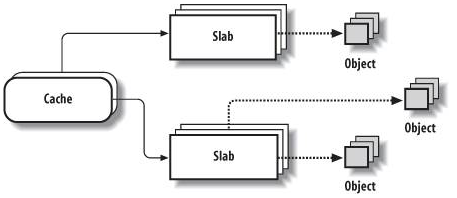
\includegraphics[keepaspectratio,width=0.3\paperwidth]{Pictures/Kernel/LinuxSlabAllocator.png}
		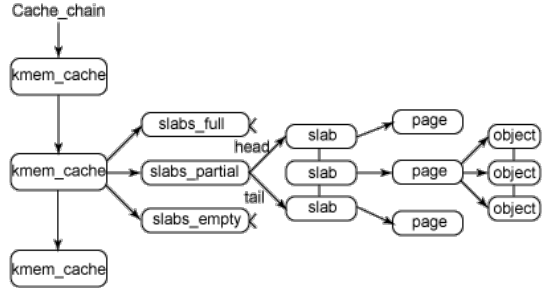
\includegraphics[keepaspectratio,width=0.3\paperwidth]{Pictures/Kernel/LinuxKmemSlab.png}
		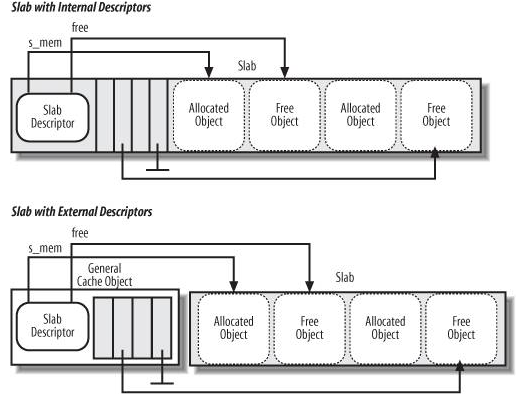
\includegraphics[keepaspectratio,width=0.3\paperwidth]{Pictures/Kernel/SlabAndObjects.png}
	    \caption{Linux内核slab分配器结构}
	\label{fig:LinuxSlabAllocator}
	\end{center}
\end{figure}



Memcached用slab分配器作内存管理。注意网上谈论的slab分配器多是memcached的分配器,而不是Linux内核的。
\begin{figure}[ht]
	\begin{center}
		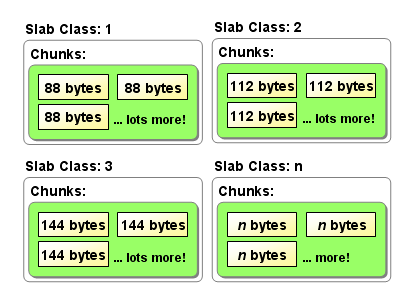
\includegraphics[keepaspectratio,width=0.3\paperwidth]{Pictures/Kernel/slabAndChunk.png}
	\caption{Memcached:slab和chunk}
	\label{fig:slabAndChunk}
	\end{center}
\end{figure}




与传统的内存管理模式相比,slab缓存分配器提供了很多优点。首先,内核通常依赖于对小对象的分配,它们会在系统生命周期内进行无数次分配。slab缓存分配器通过对类似大小的对象进行缓存而提供这种功能,从而避免了常见的碎片问题。slab分配器还支持通用对象的初始化,从而避免了为同一目而对一个对象重复进行初始化。最后,slab分配器还可以支持硬件缓存对齐和着色,这允许不同缓存中的对象占用相同的缓存行,从而提高缓存的利用率并获得更好的性能。


Linux内核中,slab分配器具体用法可以这样:
\begin{lstlisting}[language=C++]
struct kmem_cache *cachep = NULL;
cachep = kmem_cache_create("cache_name", 
  sizeof(struct mystruct), 0, SLAB_HWCACHE_ALIGN, NULL, NULL);
struct yourstruct *bodyp = NULL;
bodyp = (struct yourstruct *) kmem_cache_alloc(cachep, 
  GFP_ATOMIC & ~__GFP_DMA);
// .... use bodyp
kmem_cache_free(cachep, bodyp);
// .... other stuff
kmem_cache_destroy(cachep);
\end{lstlisting}


proc文件系统提供了一种简单的方法来监视系统中所有活动的 slab 缓存。这个文件称为 /proc/slabinfo,
它除了提供一些可以从用户空间访问的可调整参数之外,还提供了有关所有slab缓存的详细信息。
要调优特定的slab缓存,可以简单地向 /proc/slabinfo 文件中以字符串的形式回转slab缓存名称和3个可调整的参数。
格式为 “cacheName limit batchcount sharedfactor”:
\begin{verbatim}
# echo "my_cache 128 64 8" > /proc/slabinfo
\end{verbatim}
limit字段表示每个CPU可以缓存的对象的最大数量。
batchcount字段是当缓存为空时转换到每个CPU缓存中全局缓存对象的最大数量。sharedfactor参数说明了SMP系统的共享行为。





Linux内核之内存管理
\url{http://www.360doc.com/content/13/0414/15/7044580_278199905.shtml}

\subsection{slab, slub和slob}

Slab是基础,是最早从Sun OS那引进的;Slub是在Slab上进行的改进,在大型机上表现出色;而Slob(Simple List Of Blocks)是针对小型系统设计的,主要是嵌入式。


SLAB是Linux上一个古老的内存分配器。因为其结构复杂,所以几乎没有人敢修改它。
众所周知,操作系统进行内存分配的时候,是以页为单位进行的,也可以称为内存块或者堆。但是内核对象远小于页的大 小,而这些对象在操作系统的生命周期中会被频繁的申请和释放,并且实验发现,这些对象初始化的时间超过了分配内存和释放内存的总时间,所以需要一种更细粒 度的针对内核对象的分配算法,于是SLAB诞生了:
SLAB缓存已经释放的内核对象,以便下次申请时不需要再次初始化和分配空间,类似对象池的概念。并且没有修改通用的内存分配算法,以保证不影响大内存块分配时的性能。

SLAB最上层为一个由多个kmem\_cache组成的cache chain。
每个kmem\_cache由slabs\_full,slabs\_partial,slabs\_empty这3个队列组成,分别标记slab全部已被分配的 页,部分被分配的页,为分配slab的页。显然,一个新的slab申请到达时,slab\_partial页会被考虑;一个内存块释放时, slab\_empty将被优先考虑。

由于SLAB按照对象的大小进行了分组,在分配的时候不会产生堆分配方式的碎片,也不会产生Buddy分配算法中的空间浪费,并且支持硬件缓存对齐来提高TLB的性能,堪称完美。
但是这个世界上没有完美的算法,一个算法要么占用更多的空间以减少运算时间,要么使用更多的运算时间减少空间的占用。优秀的算法就是根据实际应用情况在这 两者之间找一个平衡点。SLAB虽然能更快的分配内核对象,但是metadata,诸如缓存队列等复杂层次结构占用了大量的内存。

SLUB("the unqueued slab allocator") 因此而诞生:
SLUB 不包含SLAB这么复杂的结构。SLAB不但有队列,而且每个SLAB开头保存了该SLAB对象的metadata。SLUB只将相近大小的对象对齐填入页面,并且保存了未分配的SLAB对象的链表,访问的时候容易快速定位,省去了队列遍历和头部metadata的偏移计算。该链表虽然和SLAB一样是每 CPU节点单独维护,但使用了一个独立的线程来维护全局的SLAB对象,一个CPU不使用的对象会被放到全局的partial队列,供其他CPU使用,平 衡了个节点的SLAB对象。回收页面时,SLUB的SLAB对象是全局失效的,不会引起对象共享问题。另外,SLUB采用了合并相似SLAB对象的方法, 进一步减少内存的占用。

据内核开发人员称,SLUB相对于SLAB有5\%-10\%的性能提升和减少50\%的内存占用。所以SLUB是一个时间和空间上均有改善的算法,而且SLUB完全兼容SLAB的接口,所以内核其他模块不需要修改即可从SLUB的高性能中受益。SLUB在2.6.22内核中理所当然的替代了SLAB。

SLAB 分配器多年以来一直位于 Linux 内核的内存管理部分的核心地带,内核黑客们一般不愿意主动去更改它的代码,因为它实在是非常复杂,而且在大多数情况下,它的工作完成的相当不错。但是,随着大规模多处理器系统和 NUMA系统的广泛应用,SLAB 分配器逐渐暴露出自身的严重不足:
1. 较多复杂的队列管理。在 SLAB 分配器中存在众多的队列,例如针对处理器的本地对象缓存队列,slab 中空闲对象队列,每个 slab 处于一个特定状态的队列中,甚至缓冲区控制结构也处于一个队列之中。有效地管理这些不同的队列是一件费力且复杂的工作。

2. slab 管理数据和队列的存储开销比较大。每个 slab 需要一个 struct slab 数据结构和一个管理所有空闲对象的 kmem\_bufctl\_t(4 字节的无符号整数)的数组。当对象体积较少时,kmem\_bufctl\_t 数组将造成较大的开销(比如对象大小为32字节时,将浪费 1/8 的空间)。为了使得对象在硬件高速缓存中对齐和使用着色策略,还必须浪费额外的内存。同时,缓冲区针对节点和处理器的队列也会浪费不少内存。测试表明在一个 1000 节点/处理器的大规模 NUMA 系统中,数 GB 内存被用来维护队列和对象的引用。

3. 缓冲区内存回收比较复杂。

4. 对 NUMA 的支持非常复杂。SLAB 对 NUMA 的支持基于物理页框分配器,无法细粒度地使用对象,因此不能保证处理器级缓存的对象来自同一节点。

5. 冗余的 Partial 队列。SLAB 分配器针对每个节点都有一个 Partial 队列,随着时间流逝,将有大量的 Partial slab 产生,不利于内存的合理使用。

6. 性能调优比较困难。针对每个 slab 可以调整的参数比较复杂,而且分配处理器本地缓存时,不得不使用自旋锁。

7. 调试功能比较难于使用。

为了解决以上 SLAB 分配器的不足之处,内核开发人员 Christoph Lameter 在 Linux 内核 2.6.22 版本中引入一种新的解决方案:SLUB 分配器。
SLUB 分配器特点是简化设计理念,同时保留 SLAB 分配器的基本思想:每个缓冲区由多个小的 slab 组成,每个 slab 包含固定数目的对象。SLUB 分配器简化了kmem\_cache,slab 等相关的管理数据结构,摒弃了SLAB 分配器中众多的队列概念,并针对多处理器、NUMA 系统进行优化,从而提高了性能和可扩展性并降低了内存的浪费。为了保证内核其它模块能够无缝迁移到 SLUB 分配器,SLUB 还保留了原有 SLAB 分配器所有的接口 API 函数。


\subsection{Bélády's anomaly}
所谓\textbf{Belady}现象是指:采用FIFO算法(选择装入最早的页面置换)时,如果对—个进程未分配它所要求的全部页面,有时就会出现分配的页面数增多但缺页率反而提高的异常现象。
原因是,增加了页帧后,本应丢失的帧被命中,但逐渐移到队头,而不是追加到队尾,改变了各帧的相对顺序,后果比较复杂。












\clearpage


%!Mode:: "TeX:UTF-8"
\section{线程安全与可重入性}

\subsection{线程安全}
如果一段代码是\textbf{线程安全}的,那么多个线程在同时执行它时能确保逻辑正确。

维基百科为线程安全程度分为三类:线程安全,有条件线程安全(conditionally thread safe)和线程不安全。
有条件线程安全指对不同对象的并发访问是安全的,对共享对象的访问需被保护以防竞跑(Race)。

有两类策略可用来消除数据竞跑以达到线程安全。
第一类策略致力于消除共享状态:
\begin{itemize}
\item 代码要做到可重入:部分执行后可被重新执行,并能确保原执行正确结束。
状态信息应保存于每次“执行”的本地,一般在栈上。所有非本地状态必须通过原子操作访问,并且数据结构须为可重入的。
\item 使用线程本地存储(Thread-local storage)。
\end{itemize}
第二类策略用于共享状态无法避免的情形,依赖于同步操作,包括互斥锁、原子操作、immutable对象等。
\begin{quotation}
引入自旋锁的隐患包括死锁、“活锁”和资源饥饿。
\end{quotation}

大多数Unix函数是线程安全的(malloc,free,printf),只有少数例外,如rand,asctime,ctime,strtok,gethostbyaddr,gethostbyname,inet\_ntoa。
Unix为大多数线程不安全函数提供了可重入版本,用\_r作为后缀。

\cite{csapp}总结了四类线程不安全函数:
\begin{enumerate}
\item 不保护共享变量的函数。可用同步操作来改进,不用改变原有接口。
\item 保存多次调用间的状态的函数,如stdlib.h的rand()和string.h的strtok()。
	如欲改进必须改变原接口,让调用间状态作为参数传入下一次调用,如非标准的rand\_r()和strtok\_r()。
\item 返回指向静态变量指针的函数,如ctime(), gethostbyname()。
有两种改进策略,一是改变原有接口,让调用者传入额外参数存放返回值,如ctime\_r(), gethostbyname\_r();
二是使用lock-and-copy策略再次封装。
\item 调用线程不安全函数的函数,\textbf{可能}会成为线程不安全函数。
\cite{csapp}认为如果调用了1型或3型线程不安全函数,可以在本函数中增加同步操作wrapper,使本函数做到线程安全。
我认为此举的前提是被调用的不安全函数不会在他处被调用。
\end{enumerate}


\subsection{可重入性}
 可重入概念是在单线程操作系统的时代提出的。
 一段程序或例程是可重入的,如果它能在执行完成之前被打断并作重新调用(重入),当重入的调用完成后原调用能够正确地恢复执行。
一段程序的重入,可能由于自身原因,如执行了jmp或者call,类似于子程序的递归调用;
或者由于硬件中断,UNIX系统的signal的处理,即子程序被中断处理程序或者signal处理程序调用。
重入的子程序,按照后进先出线性序依次执行。

中断服务例程必须是可重入的,它们通常被禁止访问文件系统,甚至不允许分配内存。
直接或间接执行递归的函数也需要是可重入的。

可重入性不同于幂等性(Idempotence, $f(f(x))=f(x)$)。

可重入程序可用于实现线程安全,《CSAPP》认为可重入程序是线程安全程序的真子集,但维基百科认为可重入程序未必是线程安全的,例如下面这个程序。
这是因为不同文献对可重入性的定义不同。
\begin{lstlisting}[language=C++]    
int t;
 
void swap(int *x, int *y)
{
    int s;
 
    s = t; // save global variable
    t = *x;
    *x = *y;
 
    // hardware interrupt might invoke isr() here!
    *y = t;
    t = s; // restore global variable
}
 
void isr()
{
    int x = 1, y = 2;
    swap(&x, &y);
}
\end{lstlisting}




若一个函数是可重入的,则该函数:
\begin{itemize}
\item 最好不要含有静态(全局)非常量数据,除非是通过原子操作访问。
\item 最好不要修改自身代码,除非对自身的代码有私有拷贝。
\item 不能调用(call)不可重入的函数(有呼叫(call)到的函数需满足前述条件)。
\end{itemize}


 下述例子是线程安全的,但不是可重入的:
\begin{lstlisting}[language=C++]    
int function()
{
 mutex_lock();
 ...
 function body
 ...
 mutex_unlock();
}
\end{lstlisting}

 
 
 \subsection{线程安全计数器类的实现\cite{wikipedia}}
以下Java代码为线程安全的:
\begin{lstlisting}[language=Java]  
class Counter {
    private int i = 0; 
    public synchronized void inc() {
        i++;
    }
}
\end{lstlisting}

以下C代码为线程安全的,但不可重入。如果本代码用于一个中断handler中,执行过程中再次发生中断,则第二次调用将永远旋住。
\begin{lstlisting}[language=C]    
#include <pthread.h>
 
int increment_counter ()
{
	static int counter = 0;
	static pthread_mutex_t mutex = PTHREAD_MUTEX_INITIALIZER;
 
	pthread_mutex_lock(&mutex); 
	// only allow one thread to increment at a time
	++counter;
	// store value before any other threads increment it further
	int result = counter; 
	pthread_mutex_unlock(&mutex);
 
	return result;
}
\end{lstlisting}

以下代码用C++的原子类型作无锁实现,为线程安全、可重入的:
\begin{lstlisting}[language=C++]    
#include <atomic>
 
int increment_counter ()
{
	static std::atomic<int> counter(0); 
	int result = ++counter; 
	return result;
}
\end{lstlisting}

 
 
 
 
 \subsection{Java中的线程安全}
对于 Java 类中常见的线程安全性级别,没有一种分类系统可被广泛接受。
Joshua Bloch给出了描述五类线程安全性的分类方法:
\begin{description}
\item[不可变]不可变的对象一定是线程安全的,并且永远也不需要额外的同步。
因为一个不可变的对象只要构建正确,其外部可见状态永远也不会改变,永远也不会看到它处于不一致的状态。
Java 类库中大多数基本数值类如 Integer 、 String 和 BigInteger 都是不可变的。
\item[线程安全]“线程安全”是很严格的,不管运行时环境如何排列,线程都不需要任何额外的同步。
Java的Vector、HashTable都不满足线程安全。
\item[有条件线程安全]有条件的线程安全类对于单独的操作可以是线程安全的,但是某些操作序列可能需要外部同步。
条件线程安全的最常见的例子是遍历由 Hashtable 或者 Vector 或者返回的迭代器。
由这些类返回的由这些类返回的 fail-fast 迭代器假定在迭代器进行遍历的时候底层集合不会有变化。
为了保证其他线程不会在遍历的时候改变集合,进行迭代的线程应该确保它是独占性地访问集合以实现遍历的完整性。
\item[线程兼容]线程兼容类不是线程安全的,但是可以通过正确使用同步而在并发环境中安全地使用。
这可能意味着用一个 synchronized 块包围每一个方法调用,或者创建一个包装器对象,其中每一个方法都是同步的。
\item[线程对立]线程对立类是那些不管是否调用了外部同步都不能在并发使用时安全地呈现的类。
线程对立很少见,当类修改静态数据,而静态数据会影响在其他线程中执行的其他类的行为,这时通常会出现线程对立。
\end{description}
这种系统有其局限性:各类之间的界线不是百分之百地明确,而且有些情况它没照顾到。 
 
\subsection{C++ 的线程安全}
在STL容器(和大多数厂商的愿望)里对多线程支持的黄金规则已经由SGI定义,并且在它们的STL网站上发布。
在访问不同对象的时候无需加锁,对共享对象并发读取时也是安全的。
但多个线程对共享对象进行读、写时,STL的用户必须自行执行保护。
 
 \subsection{False sharing问题}
在做多线程程序的时候,为了避免使用锁,我们通常会采用这样的数据结构:根据线程的数目,安排一个数组, 每个线程一个项,互相不冲突。
从逻辑上看这样的设计无懈可击,但是实践的过程我们会发现这样并没有提高速度。
问题在于cpu的cache line. 我们在读主存的时候,数据同时被读到L1,L2中去,而且在L1中是以cache line(通常64)字节为单位的。
每个Core都有自己的L1,L2,所以每个线程在读取自己的项的时候, 也把别人的项读进去, 所以在别人的项更新的时候,为了保持数据的一致性, core之间cache要进行同步, 这个会导致严重的性能问题. 这就是所谓的False sharing问题 。
\begin{lstlisting}[language=C++]                      
typedef union {
    erts_smp_rwmtx_t rwmtx;
    byte cache_line_align__[ERTS_ALC_CACHE_LINE_ALIGN_SIZE(
                                sizeof(erts_smp_rwmtx_t))];
} erts_meta_main_tab_lock_t;
\end{lstlisting}

或者:
\begin{lstlisting}[language=C++]                      
_declspec (align(64)) int thread1_global_variable;
__declspec (align(64)) int thread2_global_variable;
\end{lstlisting}
 
 









%!Mode:: "TeX:UTF-8"
\section{同步保护}

\subsection{读-改-写(read-modify-write)}
读改写操作包括TestAndSet, FetchAndAdd, and CompareAndSwap(CAS)等原子操作,能够在多线程程序中消除竞跑,用于实现互斥锁、信号量,以及无锁、无等待算法。
TestAndSet的consensus numbers为2,而CAS的consensus numbers为无穷大。

TestAndSet操作在旧值为0时将其置1,不论成功与否均返回旧值。

load-link and store-conditional (LL/SC)是一对操作,LL加载某内存值,随后SC试图在该内存处写入,仅当该处在两个操作之间未发生过更新时才成功。

FetchAndAdd的行为类似于:
\begin{lstlisting}[language=C++]
<< atomic >>
function FetchAndAdd(address location, int inc) {
    int value := *location
    *location := value + inc
    return value
}
\end{lstlisting}


\subsection{互斥锁的实现}

加锁操作可用原子TestAndSet操作实现:
\begin{lstlisting}[language=C++]
function Lock(boolean *lock)
{
    while (TestAndSet(lock) == 1);
}
\end{lstlisting}

基于TestAndSet操作实现临界区保护:
(\url{http://en.wikipedia.org/wiki/Test-and-set})
\begin{lstlisting}[language=C++]
volatile int lock = 0;

void Critical() {
    while (TestAndSet(&lock) == 1);
    critical section // only one process can be in this section at a time
    lock = 0 // release lock when finished with the critical section
}
\end{lstlisting}

频繁地调用TestAndSet非常昂贵,事实上可以使用更为精细的Test-and-TestAndSet技巧来实现优化:仅当普通读操作认为未上锁时才执行原子操作。
\begin{lstlisting}[language=C++]
 procedure EnterCritical() {
   while ( locked == true or TestAndSet(locked) == true )
     skip // spin until locked
 }
\end{lstlisting}

基于FetchAndAdd操作可以用ticket lock算法实现互斥锁:
\begin{lstlisting}[language=C++]
record locktype {
    int ticketnumber
    int turn
 }
 procedure LockInit( locktype* lock ) {
    lock.ticketnumber := 0
    lock.turn := 0
 }
 procedure Lock( locktype* lock ) {
    int myturn := FetchAndIncrement( &lock.ticketnumber )
    while lock.turn ≠ myturn 
        skip // spin until lock is acquired
 }
 procedure UnLock( locktype* lock ) {
    FetchAndIncrement( &lock.turn )
 }
\end{lstlisting}


\subsection{内存屏障}
\label{subsec:MemBarrier}
内存屏障,也称内存栅栏,内存栅障,屏障指令等, 是一类同步屏障指令,使得CPU或编译器在对内存随机访问的操作中的一个同步点,使得此点之前的所有读写操作都执行后才可以开始执行此点之后的操作。

大多数现代计算机为了提高性能而采取乱序执行,这使得内存屏障成为必须。

语义上,内存屏障之前的所有写操作都要写入内存;内存屏障之后的读操作都可以获得同步屏障之前的写操作的结果。因此,对于敏感的程序块,写操作之后、读操作之前可以插入内存屏障。

C与C++语言中,volatile关键字意图允许内存映射的I/O操作。
这要求编译器对此的数据读写按照程序中的先后顺序执行,不能对volatile内存的读写重排序,也不能对读写进行省略(我的理解是不能从寄存器和cache中读写)。
但volatile不是内存栅栏,因为volatile内存和非volatile内存之间的相互顺序不能保证(编译器乱序)。
因为cache问题,volatile也不保证别的核看见的顺序是正确的(机器乱序)。
因此volatile变量不足以作为线程间通信的flag。
在C11和C++11之前,C/C++不处理多线程问题,volatile的有效性取决于编译器和硬件。

Java 1.5引入了新的内存模型,其volatile关键词已经能编译器乱序和机器乱序问题。
C++11标准化了原子操作,也能达到类似作用。

\subsection{无锁队列}
陈皓给出的无锁队列算法\footnote{\url{http://coolshell.cn/articles/8239.html}}:
\begin{lstlisting}[language=C++]
//这里head始终指向哨兵结点,tail只有为空时才指向哨兵。
EnQueue (x) //进队列
{
    //准备新加入的结点数据
    q = new record ();
    q->value = x;
    q->next = NULL;
 
    do {
        p = tail; //取链表尾指针的快照
    } while( CAS (p->next, NULL, q) != TRUE); //如果没有把结点链上,再试
 
    CAS (tail, p, q); //置尾结点
}

EnQueue(x) //进队列改良版,解决线程在设置尾结点前停掉的问题
{
    q = new record();
    q->value = x;
    q->next = NULL;
 
    p = tail;
    oldp = p
    do {
        while (p->next != NULL)
            p = p->next;
    } while( CAS(p.next, NULL, q) != TRUE); //如果没有把结点链在尾上,再试
 
    CAS(tail, oldp, q); //置尾结点
}

DeQueue() //出队列
{
    do{
        p = head;
        if (p->next == NULL){
            return ERR_EMPTY_QUEUE;
        }
    while( CAS(head, p, p->next) != TRUE );
    return p->next->value;
}
//其他实现参考:
//http://www.ibm.com/developerworks/cn/aix/library/au-multithreaded_structures2/index.html
//http://www.codeproject.com/Articles/153898/Yet-another-implementation-of-a-lock-free-circular
//http://www.drdobbs.com/parallel/writing-lock-free-code-a-corrected-queue/210604448?pgno=2
\end{lstlisting}








%!Mode:: "TeX:UTF-8"
\section{操作系统实例}

Unix包括:
\begin{description}
\item [AIX] IBM开发的一套UNIX操作系统
\item [Solaris] SUN公司研制的类Unix操作系统
\item [HP-UX] 惠普科技公司(HP,Hewlett-Packard)以SystemV为基础所研发成的类UNIX操作系统。
\item [IRIX] SGI)以System V与BSD延伸程序为基础所发展成的UNIX操作系统,IRIX可以在SGI公司的RISC型电脑上运行
\item [Xenix] 是一种UNIX操作系统,可在个人电脑及微型计算机上使用
\end{description}

Mac OS X使用Darwin作为系统核心,而Darwin核心是以FreeBSD为范本加以改写而成。

Linux包括OpenSuse,Gentoo,Slackware,Mandriva等。




%!Mode:: "TeX:UTF-8"
\section{Procfs和Sysfs}

\subsection{Procfs}
在许多类 Unix 计算机系统中, procfs是进程文件系统 (file system) 的缩写,包含一个伪文件系统(启动时动态生成的文件系统),用于通过内核访问进程信息。这个文件系统通常被挂载到 /proc 目录。由于 /proc 不是一个真正的文件系统,它也就不占用存储空间,只是占用有限的内存。

The proc file system acts as an interface to internal data structures in the kernel. It can be used to obtain information about the system and to change certain kernel parameters at runtime (sysctl).
The proc filesystem provides a method of communication between kernel space and user space. For example, the GNU version of ps uses the procfs to obtain its data, without using any specialized system calls.

task目录就是用来描述进程中线程的,因此也可以通过下面的方法获取某进程中运行中的线程数量(PID指的是进程ID):
\begin{verbatim}
ls /proc/PID/task | wc -l
\end{verbatim}  


\subsection{Sysfs}
Sysfs 是 Linux 2.6 所提供的一种虚拟文件系统。这个文件系统不仅可以把设备(devices)和驱动程序(drivers) 的信息从内核输出到 用户空间,也可以用来对设备和驱动程序做设置。
当时由于procfs 文件系统过度混乱,包含了许多不是进程(process)的信息, sysfs 的目的是把一些原本在 procfs 中的,关于设备的部份独立出来,以‘设备层次结构架构’(device tree)的形式呈现。
每个被加入 driver model tree 内的对象,包括驱动程序、设备以及 class 设备,都会在 sysfs 文件系统中以一个目录呈现。

Sysfs通常被加载到/sys目录。

\begin{figure}[ht]
	\begin{center}
		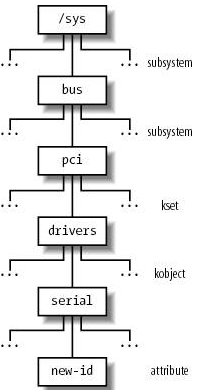
\includegraphics[keepaspectratio,width=0.3\paperwidth]{Pictures/Kernel/DeviceDriverModelHierarchyExample.png}
	\caption{驱动程序模型层次}
	\label{fig:DeviceDriverModelHierarchyExample}
	\end{center}
\end{figure}

sysfs 一开始以 ramfs 为基础,也是一个只存在于存储器中的文件系统。sysfs 刚开始被命名成 ddfs (Device Driver Filesystem),当初只是为了要对新的驱动程序模型除错而开发出来的。它在除错时,会把设备架构(device tree)的信息输出到 procfs 文件系统中。但在 Linus Torvalds 的急切督促下,ddfs 被转型成一个以 ramfs 为基础的文件系统。在新的驱动程序模型被集成进 2.5.1 核心时,ddfs 被改名成 driverfs,以更确切描述它的用途。在2.5 核心开发的次年,新的“驱动程序模型”和 "driverfs" 证明了对核心中的其他子系统也有用处。kobjects 被开发出来,作为核心对象的中央管理机制,而此时 driverfs 也被改名成 sysfs。



\clearpage

\bibliographystyle{unsrt}
\bibliography{thebib}



\end{document}
